\documentclass[../../Matt_Gebert_Honours_Thesis.tex]{subfiles}

\begin{document}
	To create graphene devices where we can measure the electronic properties referenced in \cref{sec:fet,sec:electronic_properties}, a variety of steps need to be taken in order to probe electronic flow. \Cref{fig:litho} describes the general process for exfoliated graphene (see \cref{sec:exfoliation}), the bulk of the devices.
	
	\begin{figure}[H]
	\centering
	\begin{subfigure}{0.2\textwidth}
		\centering
		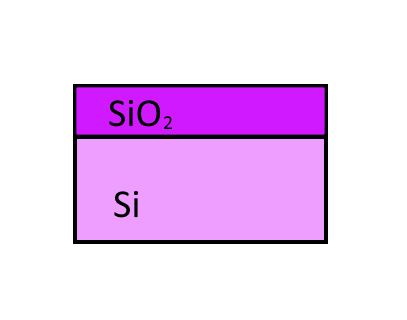
\includegraphics[width=\textwidth]{chap2/lithography/01SiliconOxide}
		\caption{Surface preparation of \silicondioxide}
	\end{subfigure}
	\hspace{0.04\textwidth}
	\begin{subfigure}{0.2\textwidth}
		\centering
		\includegraphics[width=\textwidth]{chap2/lithography/02graphene}
		\caption{Exfoliation of graphene on \silicondioxide}
	\end{subfigure}
	\hspace{0.04\textwidth}
	\begin{subfigure}{0.2\textwidth}
		\centering
		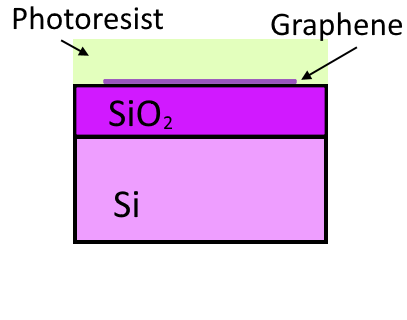
\includegraphics[width=\textwidth]{chap2/lithography/03Photoresist}
		\caption{Spin coat light sensitive photoresist}
	\end{subfigure}
	\hspace{0.04\textwidth}
	\begin{subfigure}{0.2\textwidth}
		\centering
		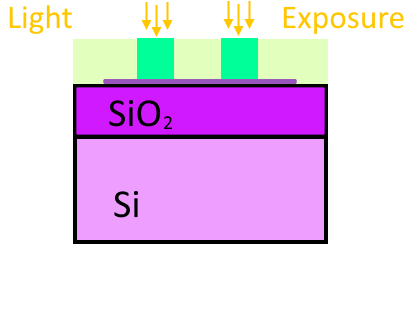
\includegraphics[width=\textwidth]{chap2/lithography/04Exposure}
		\caption{Masked exposure of photoresist to light}
	\end{subfigure}
	\end{figure}
	\begin{figure}[H]
	\centering
	\ContinuedFloat
	\begin{subfigure}{0.2\textwidth}
		\centering
		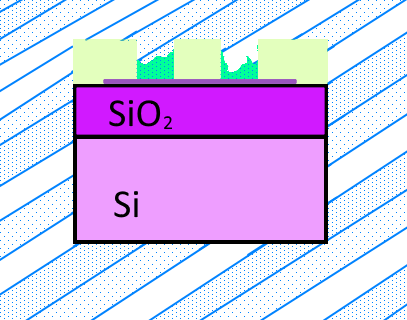
\includegraphics[width=\textwidth]{chap2/lithography/05Develop}
		\caption{Develop exposed photoresist}
	\end{subfigure}
	\hspace{0.04\textwidth}
	\begin{subfigure}{0.2\textwidth}
		\centering
		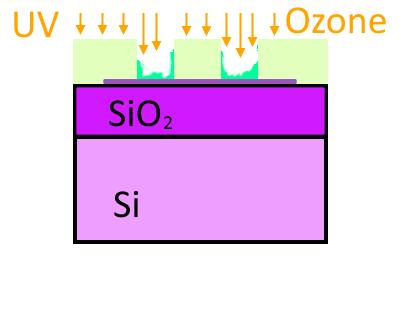
\includegraphics[width=\textwidth]{chap2/lithography/06UVOzone}
		\caption{UV Ozone Cleaning}
	\end{subfigure}
	\hspace{0.04\textwidth}
	\begin{subfigure}{0.2\textwidth}
		\centering
		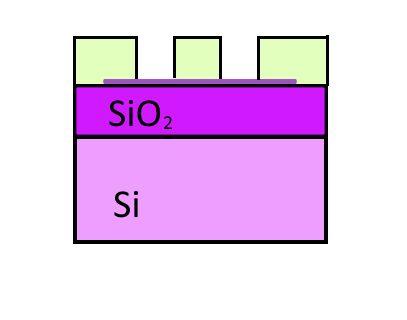
\includegraphics[width=\textwidth]{chap2/lithography/06Clean}
		\caption{After UV Ozone}
	\end{subfigure}
	\hspace{0.04\textwidth}
	\begin{subfigure}{0.2\textwidth}
		\centering
		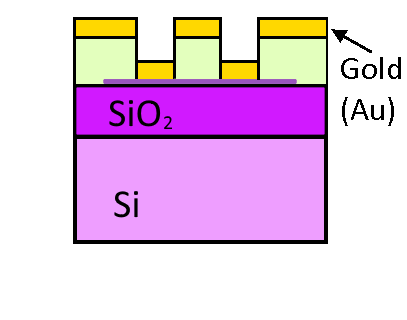
\includegraphics[width=\textwidth]{chap2/lithography/07Deposition}
		\caption{Deposition of metals}
	\end{subfigure}
	\end{figure}
	\begin{figure}[H]
	\ContinuedFloat
	\centering
	\begin{subfigure}{0.2\textwidth}
		\centering
		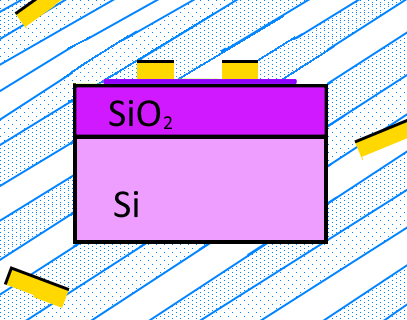
\includegraphics[width=\textwidth]{chap2/lithography/07LiftOff}
		\caption{Lift off: Removal of remaining photoresist and excess metal}
	\end{subfigure}
	\hspace{0.04\textwidth}
	\begin{subfigure}{0.2\textwidth}
		\centering
		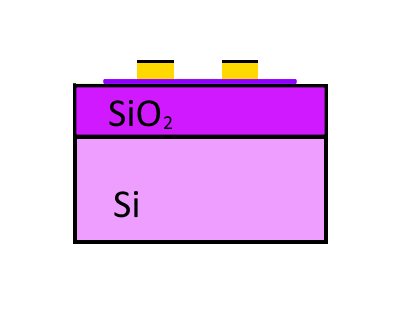
\includegraphics[width=\textwidth]{chap2/lithography/08Clean}
		\caption{Final result}
	\end{subfigure}
	\caption[Device fabrication process]{Device fabrication process from exfoliated graphene to a FET device.}\label{fig:litho}
	\end{figure}
	
	\subsection{Graphene}
	Since graphene's realisation in 2004 \cite{novoselov_electric_2004}, much research has been focused to finding effecient ways of producing large amounts of graphene \cite{zhang_review_2013}. Originally, the first samples ever created which have primarily been used for sensative measuremnts have been conducted using a method of exfoliation (\cref{sec:exfoliation}). These samples typically exhibit better electronic properties than those produced by other methods.
	Since 2008/2009, CVD (\cref{sec:CVD}) of carbon to create graphene films has provided another prominent method to produce large films for industrial scale applications. In particular, growth of graphene on copper sheets \cite{li_large-area_2009} has been a reliable way producing these large uniform sheets.
	
	There are other methods not used in this thesis, such as epitaxial growth of graphene via SiC uses heating to boil off silicon atoms to form a layer of graphene on it's surface.
	
	\subsection{Chemical vapor deposition graphene}\label{sec:CVD}
	Graphene can be growth via chemical vapor deposition, resulting in particularly large uniform sheets when grown on copper \cite{li_large-area_2009}. This is a widely used method of producing readily available graphene. Graphene produced in this fashion needs to be transfered onto an insulating layer of oxide to create a gate, or be gated by using a deposition method. We have used the former, which will introduce some cracks, folding and wrinkling disorder when transfered.
	
	\begin{wrapfigure}[17]{r}[0pt]{8cm}
		\centering
		\vspace{-0.5cm}
		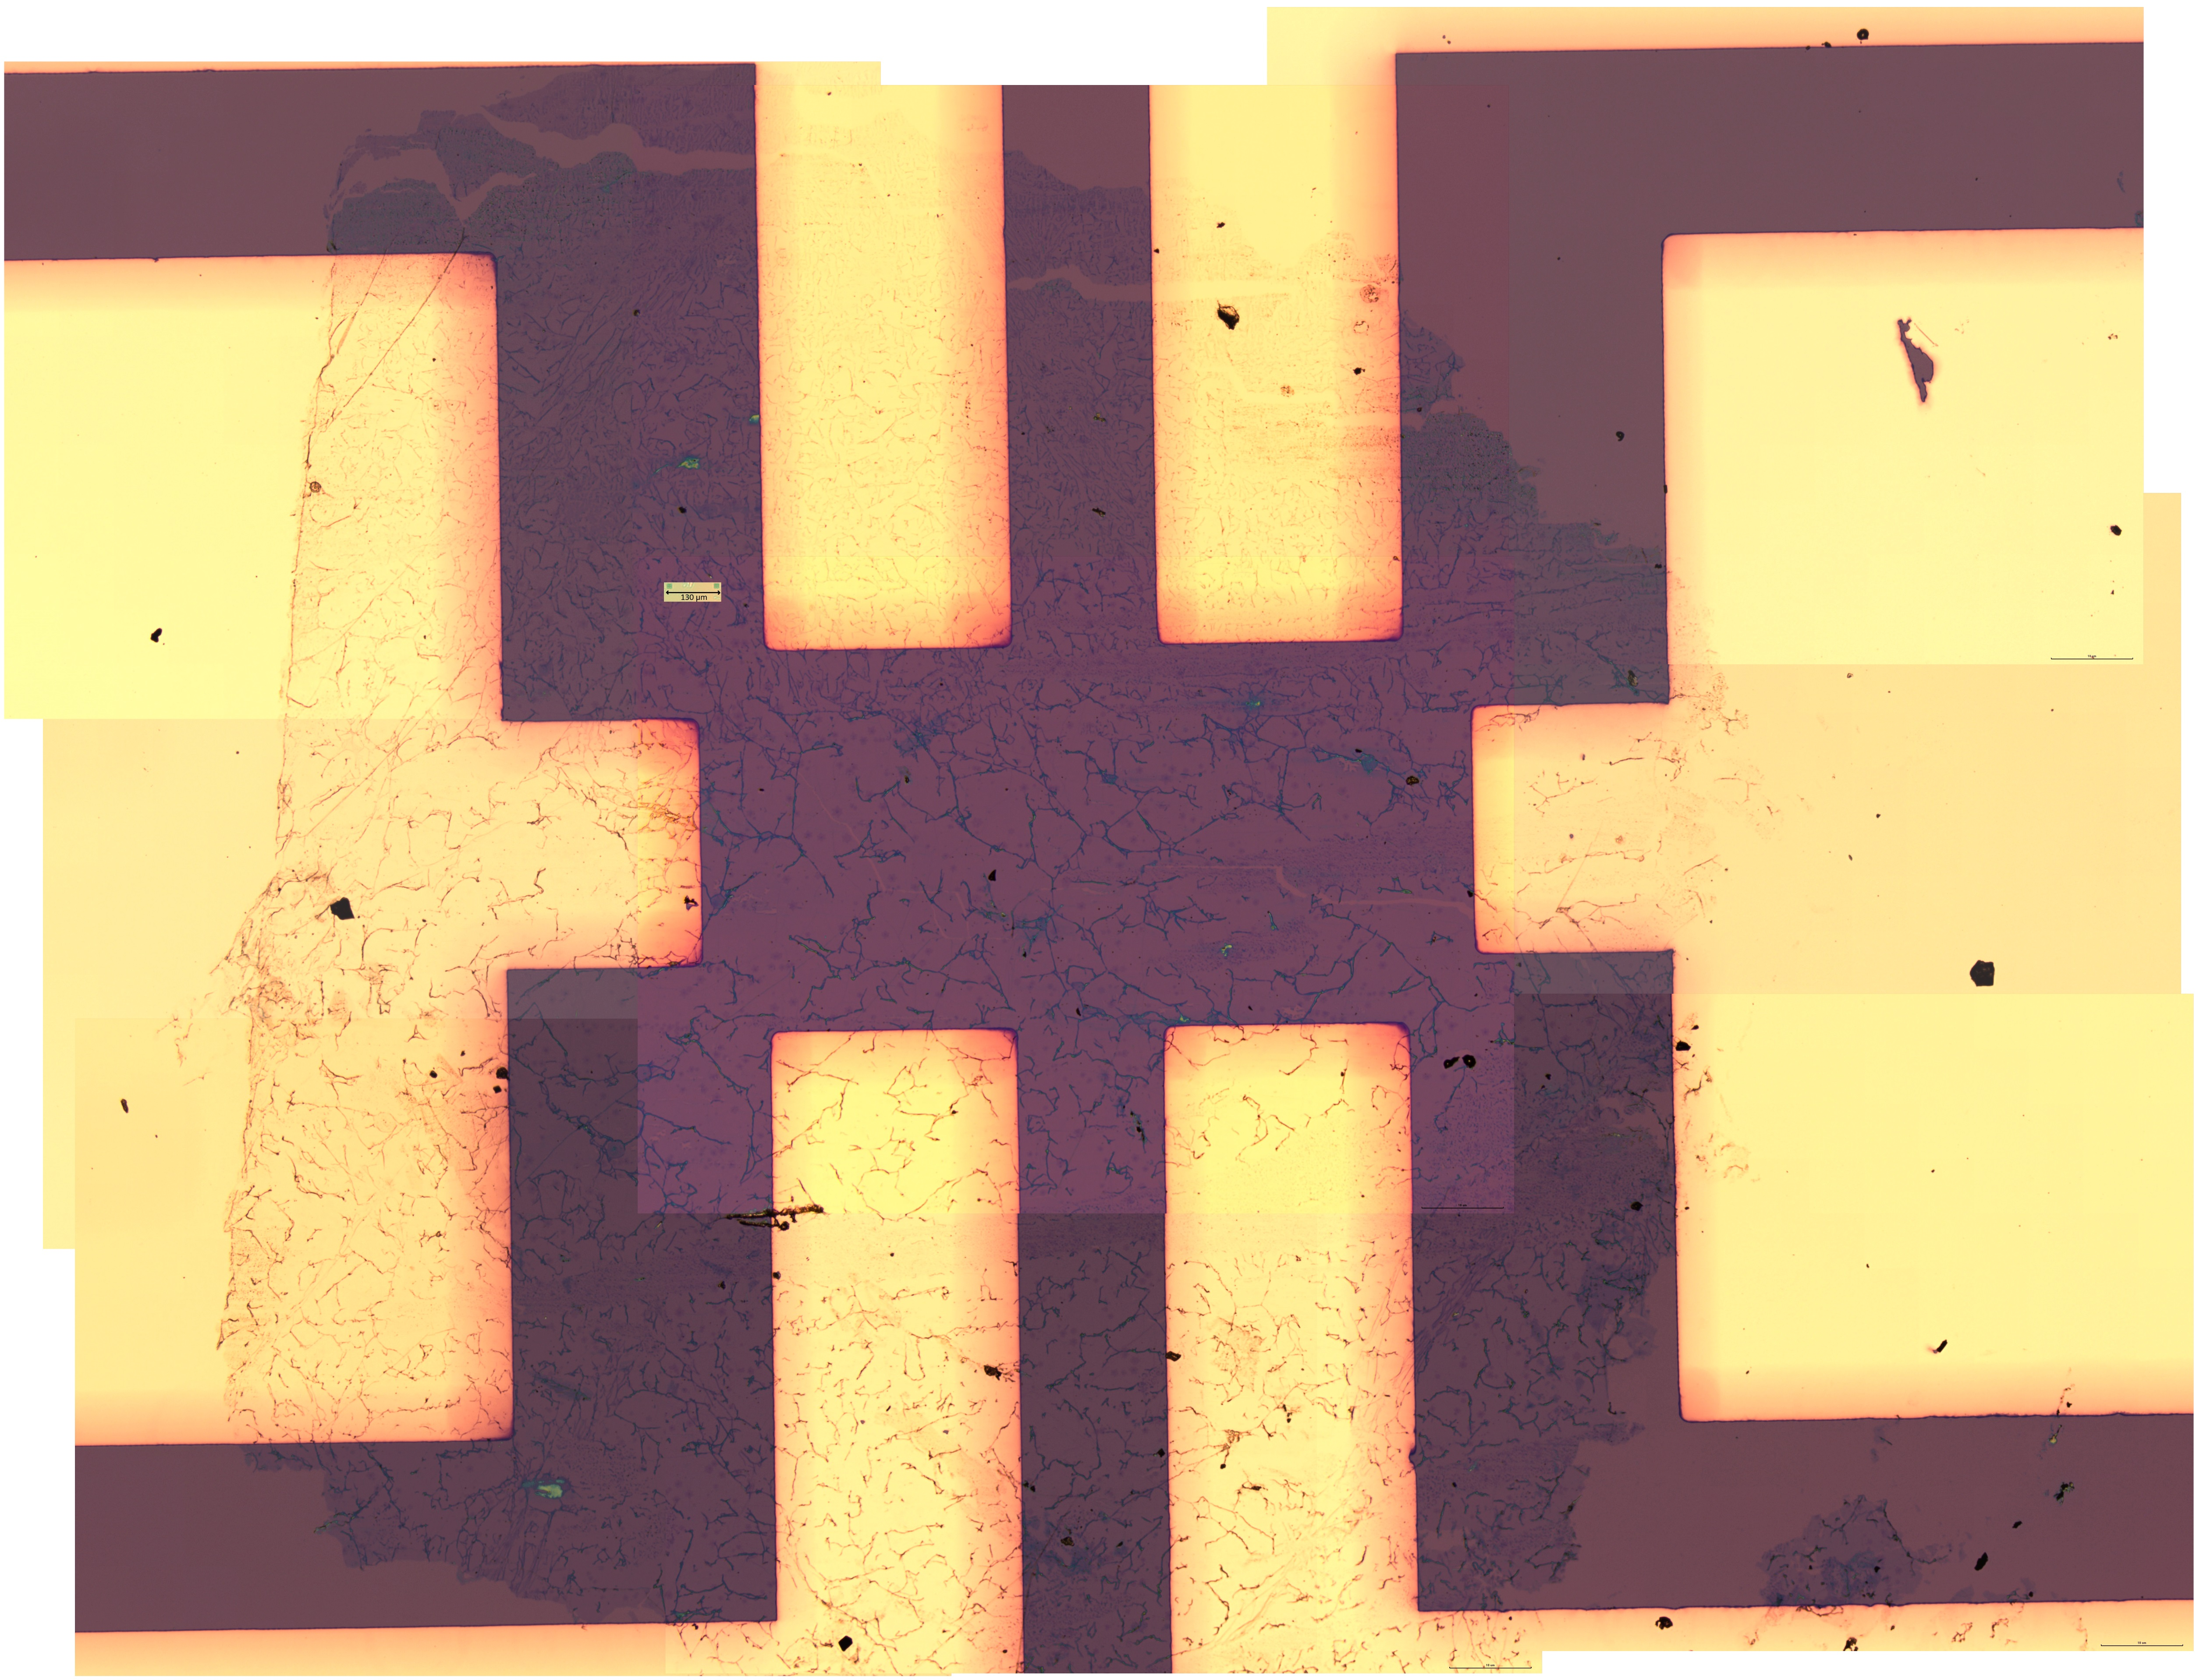
\includegraphics[width=0.5\textwidth]{chap2/cvd_graphene}
		\caption[CVD graphene grown on Cu transferred onto \silicondioxide{} and Au pads.]{CVD graphene grown on Cu transferred onto \silicondioxide{} and Au pads. The contrast differences due to the autoexposure of the camera software.} \label{fig:cvd_grpahene} 
	\end{wrapfigure}

	To achieve this, a process\cite{zheng_direct_2017} using polymethyl methacrylate (PMMA) is used to 'wet transfer' CVD graphene onto a \silicondioxide{} wafer with pre-deposited Au pads, from a masked e-beam deposition (see \cref{sec:deposition}). 
	
	Copper grown CVD graphene, covered by PMMA, is placed in an ammonium persulfate solution, dissolving the copper. The remaining graphene and PMMA remains hydrophobic on the surface, and allows substrates to collect the sample beneath. After the transfer is complete, the sample is soaked in PG remover to clean off PMMA. An example device is shown in \cref{fig:cvd_grpahene}. 
	
	We seldom used this technique to produce graphene devices due to the area coverage requirement of an oxide as well as the lack of goemetric definition.
	
	\subsection{Exfoliation of graphene}\label{sec:exfoliation}
	Exfoliation in materials refers to the cleaving thin layers (or leaves) off a larger sample, and acquiring them onto the substrate. We exfoliate graphene onto Si/SiO$_2$ wafers. 
	Generally exfoliation involves pressing tape/surfaces against a bulk crystal (such as highly orientated pyrolitic graphite (HOPG), Kish graphite, natural graphite, or graphenium). Due to van der Waals interactions, layers of graphite are transferred to the desired surface. By repeated peeling of the same tape, a thin coverage can be obtained and then transferred onto substrates, such as \silicondioxide.
	Exfoliation can take a variety of forms, from Geim's method \cite{novoselov_two-dimensional_2005}, to directly applying scotch tape to HOPG and then pressing against SiO$_2$, before peeling the tape off.
	
	Huang \etal investigated a reliable method of exfoliation to produce large area and high quality samples \cite{huang_reliable_2015}, which has been widely cited. Tape with graphite flakes is brought into contact with a silicon dioxide wafer, and an annealing process of heating the tape and wafer for 2-5m at $\sim 100^\circ$C on a conventional lab hot plate is used. After allowing cooling to room temperature, the tape is removed. They find under optical microscopy that graphene flakes with uniform thickness routinely range from $\sim 20\mu$m to above $100\mu$m. In this context, annealing is expected to increase traction due to the remove of gas moelcules trapped between SiO$_2$ and graphite.\newline 
	
	The following steps make up the process of exfoliation we optimised:
	\begin{enumerate}
		\itemsep 0em
		\item (Optional) Use a plasma asher/etcher with an argon/oxygen plasma to the clean surface of \silicondioxide. This can increase the adhesion between graphene and the surface by removing organic absorbates\cite{huang_reliable_2015}. Alternatively, clean wafers of Si/SiO$_2$ in acetone, tilted in an ultrasonic bath for 30s. Repeat the same in isopropanol, before rinsing in ethanol and drying with N$_2$ gas.
		\item Cleave a layer of HOPG graphite by using scotch tape to peel off a thick film.
		\item Use a secondary piece of scotch tape to exfoliate a thinner layer off master tape. Ensure good coverage by reattaching a couple times. 
		\item Attach Si/SiO$_2$ wafers to graphite covered areas of secondary tape. The SiO$_2$ face should be contacting the graphite.
		\item Attach the tape and wafers firmly to a glass slide, before using a tissue/cotton-bud to press the surface of the tape into the wafer.
		\item Place glass slide on a hotplate at $100^\circ$C for two minutes, before removing and cooling for two minutes.
		\item Slowly peel tape at an acute angle from the glass slide, roughly at 6s per cm over the wafer.
	\end{enumerate}
	
	We found success can depend on HOPG crystal, given we tried cleavage using ZYA and ZYB quality crystals and had repeated failure. Changing to a new ZYA crystal provided immediate results using the same process.
	
	\subsection{Lithography}\label{sec:lithography}
	Lithography can be used to create polymer structures that allow the deposition of desired material in 2D geometries. This is used to create electrical contacts onto graphene. This process and the adjustements made for fabricating our devices are described in this section.\newline
	
	Lithography typically consists of three main steps.
	\begin{enumerate}
		\itemsep0em
		\item Spin coating - covering a sample with a uniform layer of polymer, and baking it on.
		\item Exposure - The polymer undergoes chemical changes to its properties when exposed to particular wavelengths of light. This differentiates exposed areas to those unexposed.
		\item Developer solution - developer solution removes indended areas of photoresist to create structures.
	\end{enumerate}
	
	\subsubsection{Spin coating photoresists}\label{sec:resists}
	A spin coater is used to deposit thin films of materials. A vacuum holds a sample on the spinner, before drops of photoresist are introduced to the sample, which is then spun over sometime to achieve a uniform thickness of photoresist. Baking on a hotplate follows to set the photoresist layer on the sample.
	
	Photoresists vary in their spinning thickness, but also their exposure rates. Positive photoresists dissolve in particular developer solutions when exposed to light, while negative photoresists dissolve if not exposed to light. We have only used positive photoresists, as we have primarily been creating structures for deposition, and not etching material where you want the bulk of the wafer exposed.
	
	\paragraph{HMDS \& AZ-1512HS}
	Initially devices were fabricated using the AZ-1512HS polymer, with the additional use of hexamethyldisilazane (HMDS) as an adhesion promoter between SiO$_2$ and AZ-1512HS. Devices were spun initially for 10 s at 1000 rpm, before being spun between 2000 and 3000 rpm for 30 s, per resist layer. This leaves a thickness of 1.7 $\mu$m to 1.39 $\mu$m \cite{az1500_series}.
	Devices were then baked at 100 $^\circ$C for 1 minute.
	
	\begin{figure}[H]\label{fig:spin_curve_AZ-1512HS}
		\centering
		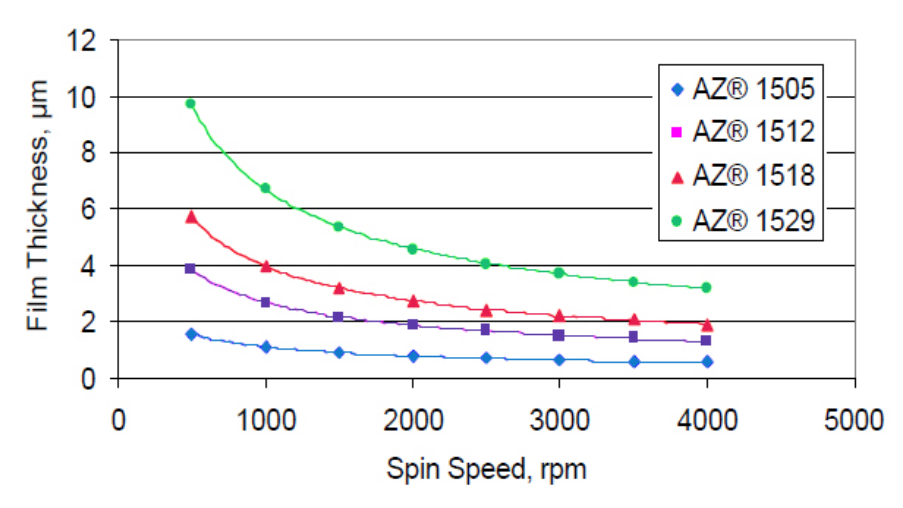
\includegraphics[width=0.7\textwidth]{chap2/az1512-spin-curve.png}
		\caption[Spin curve of AZ-1512HS]{Spin curve of AZ-1512HS (Source: EMD Performance Materials\cite{az1500_series_spincurve})}
	\end{figure}
	
	\paragraph{Skin issues with HMDS}\label{sec:skin_issues}
	When using HMDS and AZ-1512HSHS in conjunction, significant amounts of deposition remenants were found on samples as seen in \cref{fig:lithography_skins}.
	
	\begin{figure}[H]
		\centering
		\begin{subfigure}[b]{0.3\textwidth}
			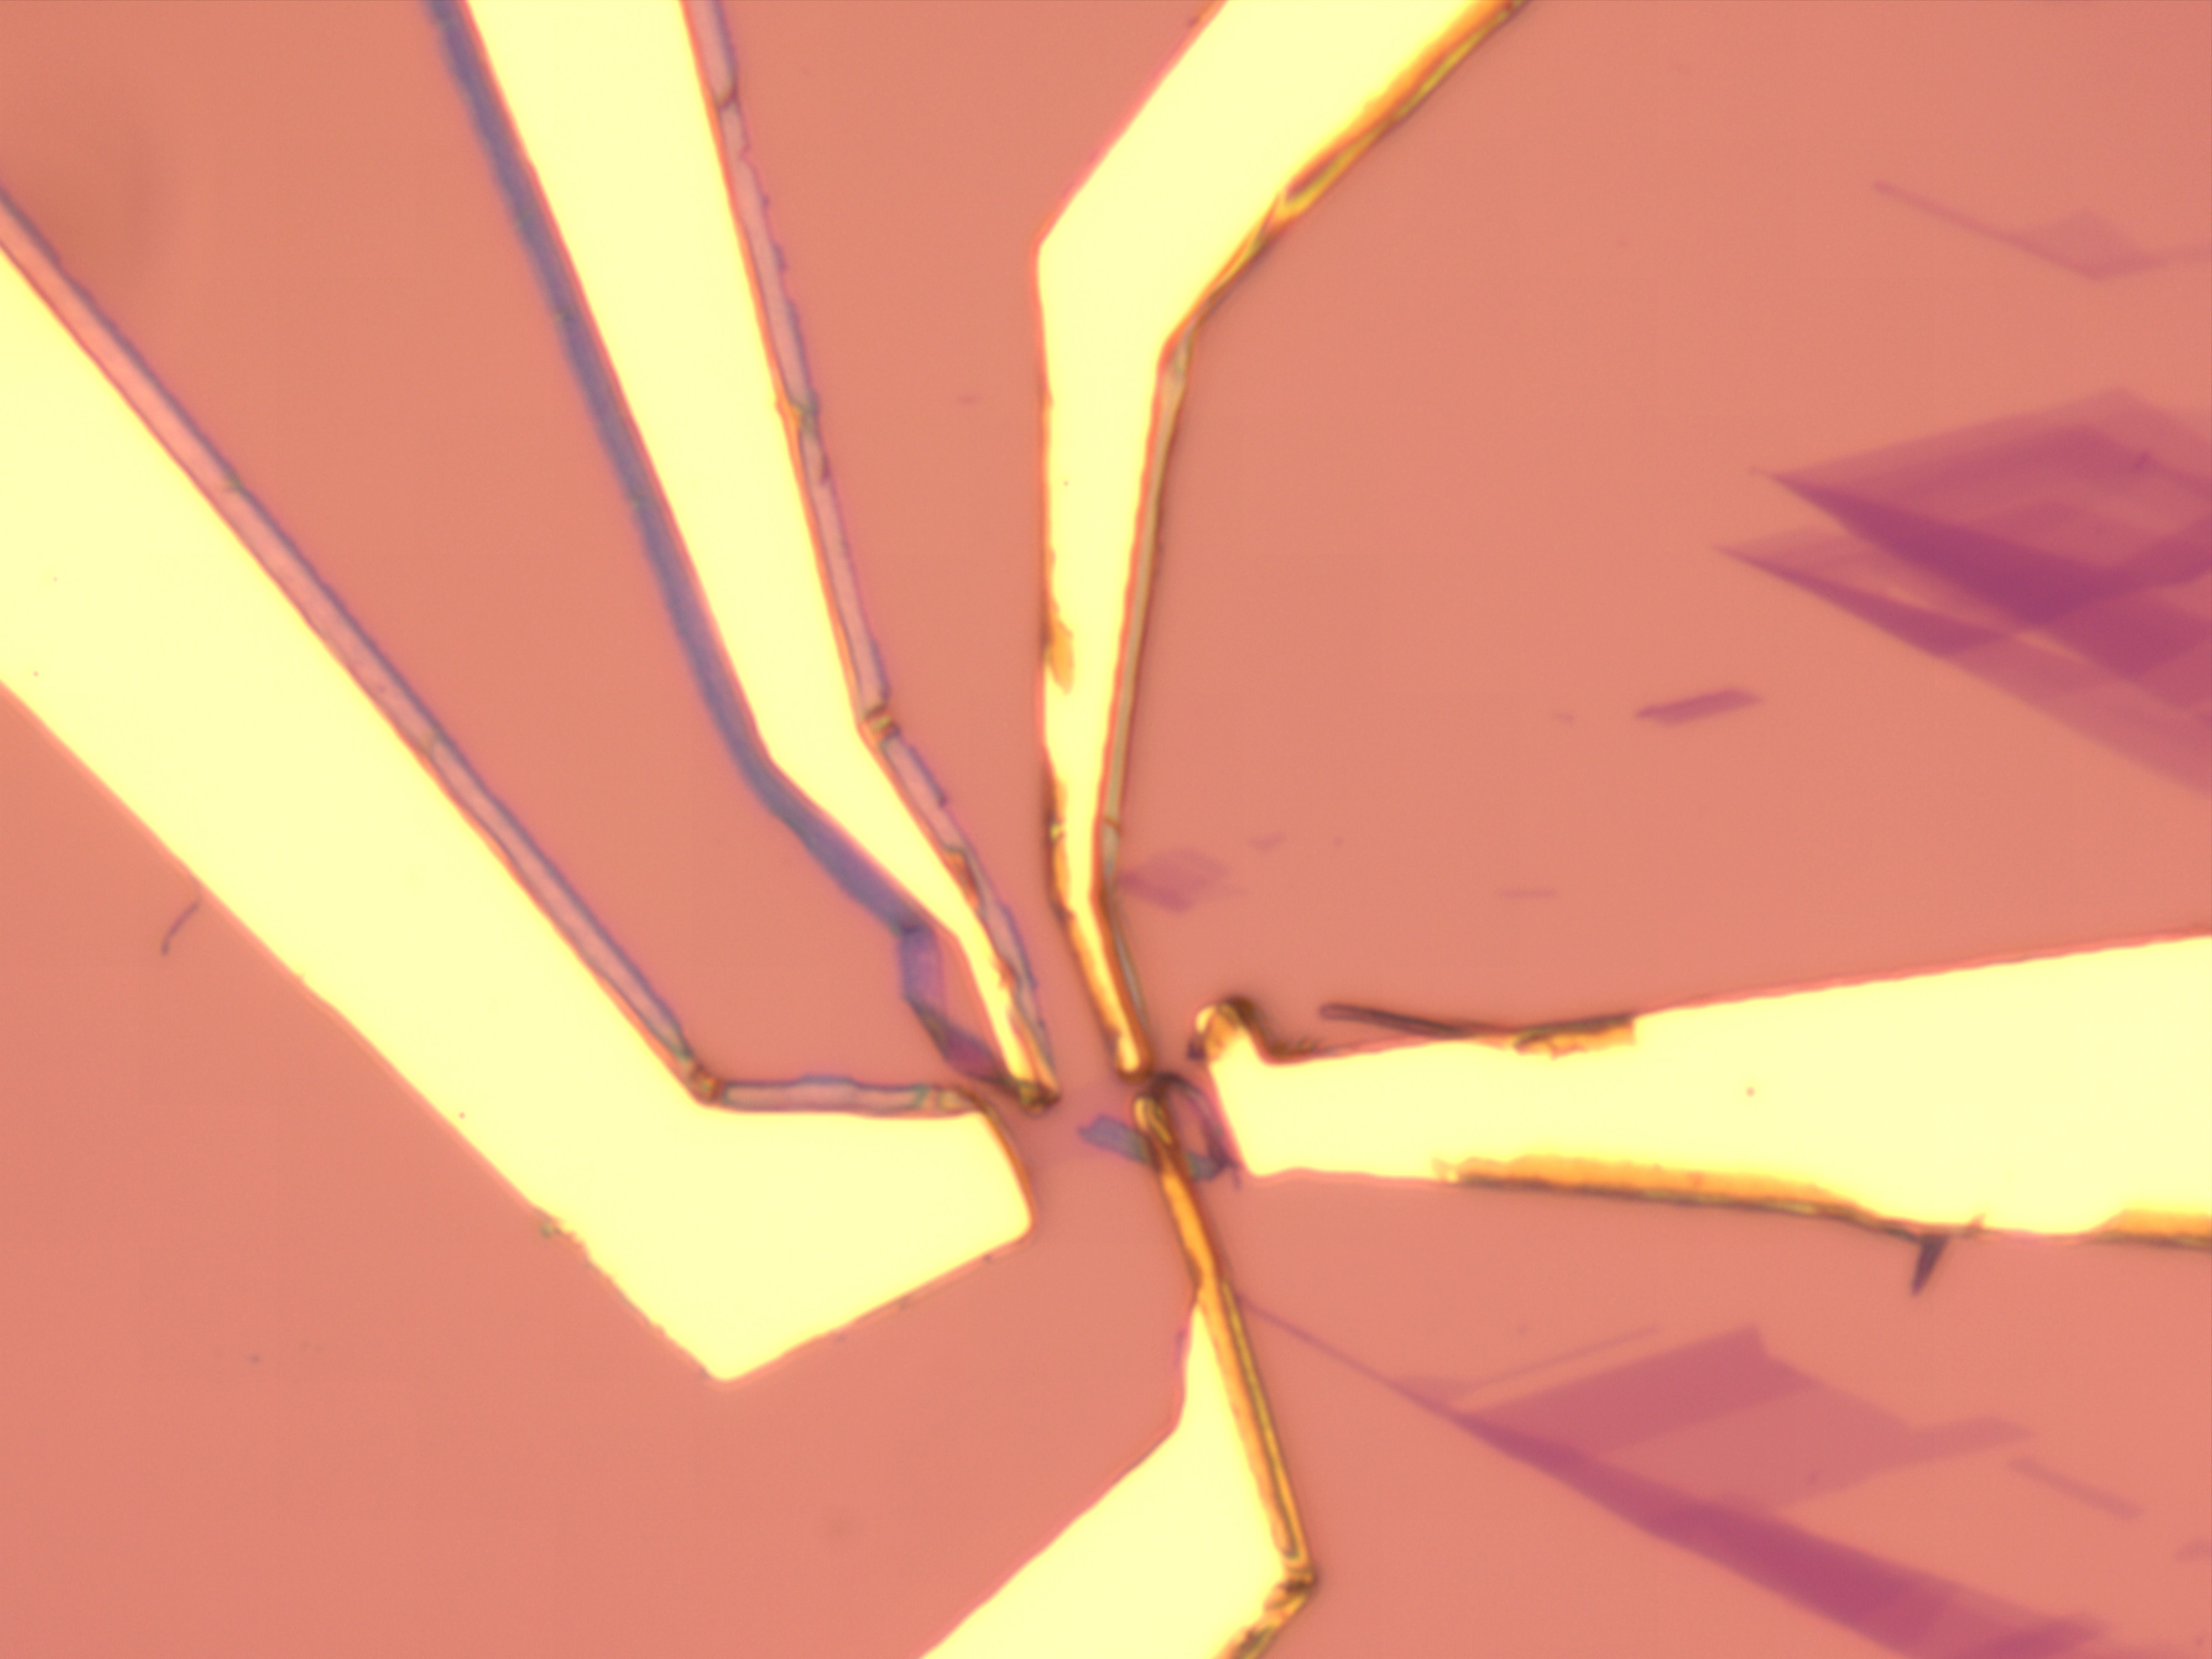
\includegraphics[width=\textwidth]{chap2/skins/Litho01_B07_WA1_F10_100x.jpg}
%			\caption{}
		\end{subfigure}
		\begin{subfigure}[b]{0.3\textwidth}
			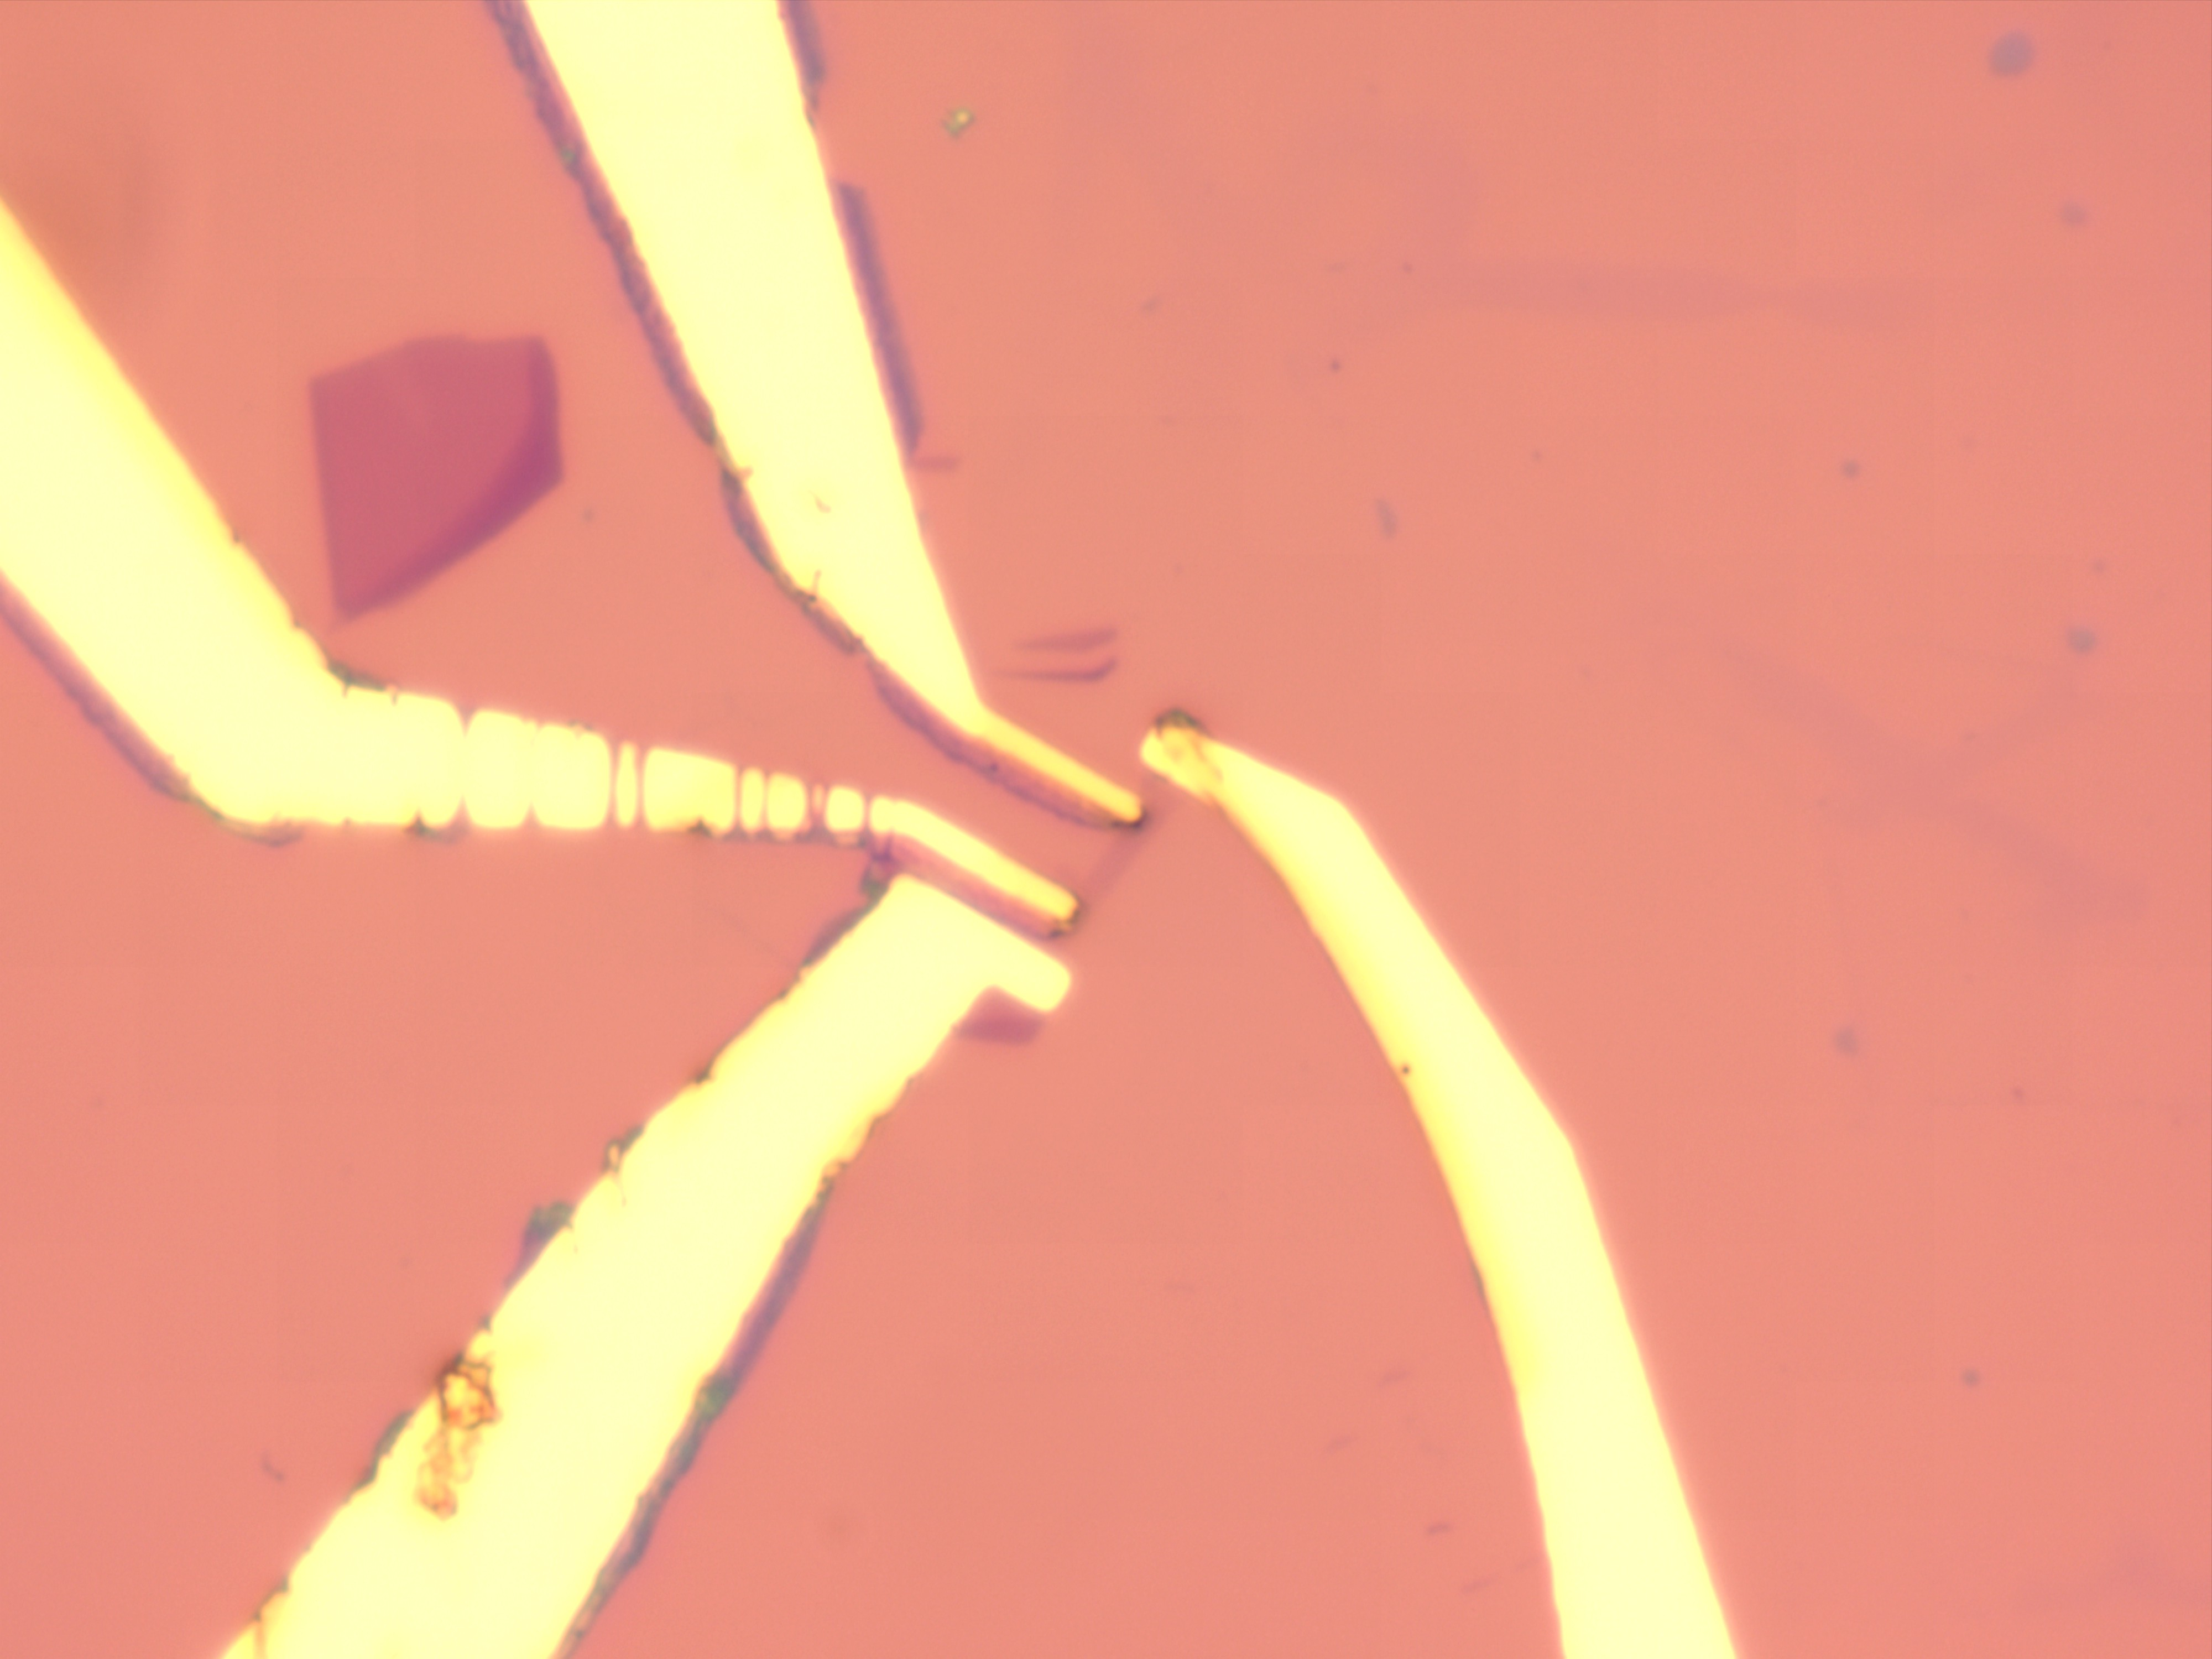
\includegraphics[width=\textwidth]{chap2/skins/1_100x.jpg}
%			\subcaption{}
		\end{subfigure}
		\begin{subfigure}[b]{0.3\textwidth}
			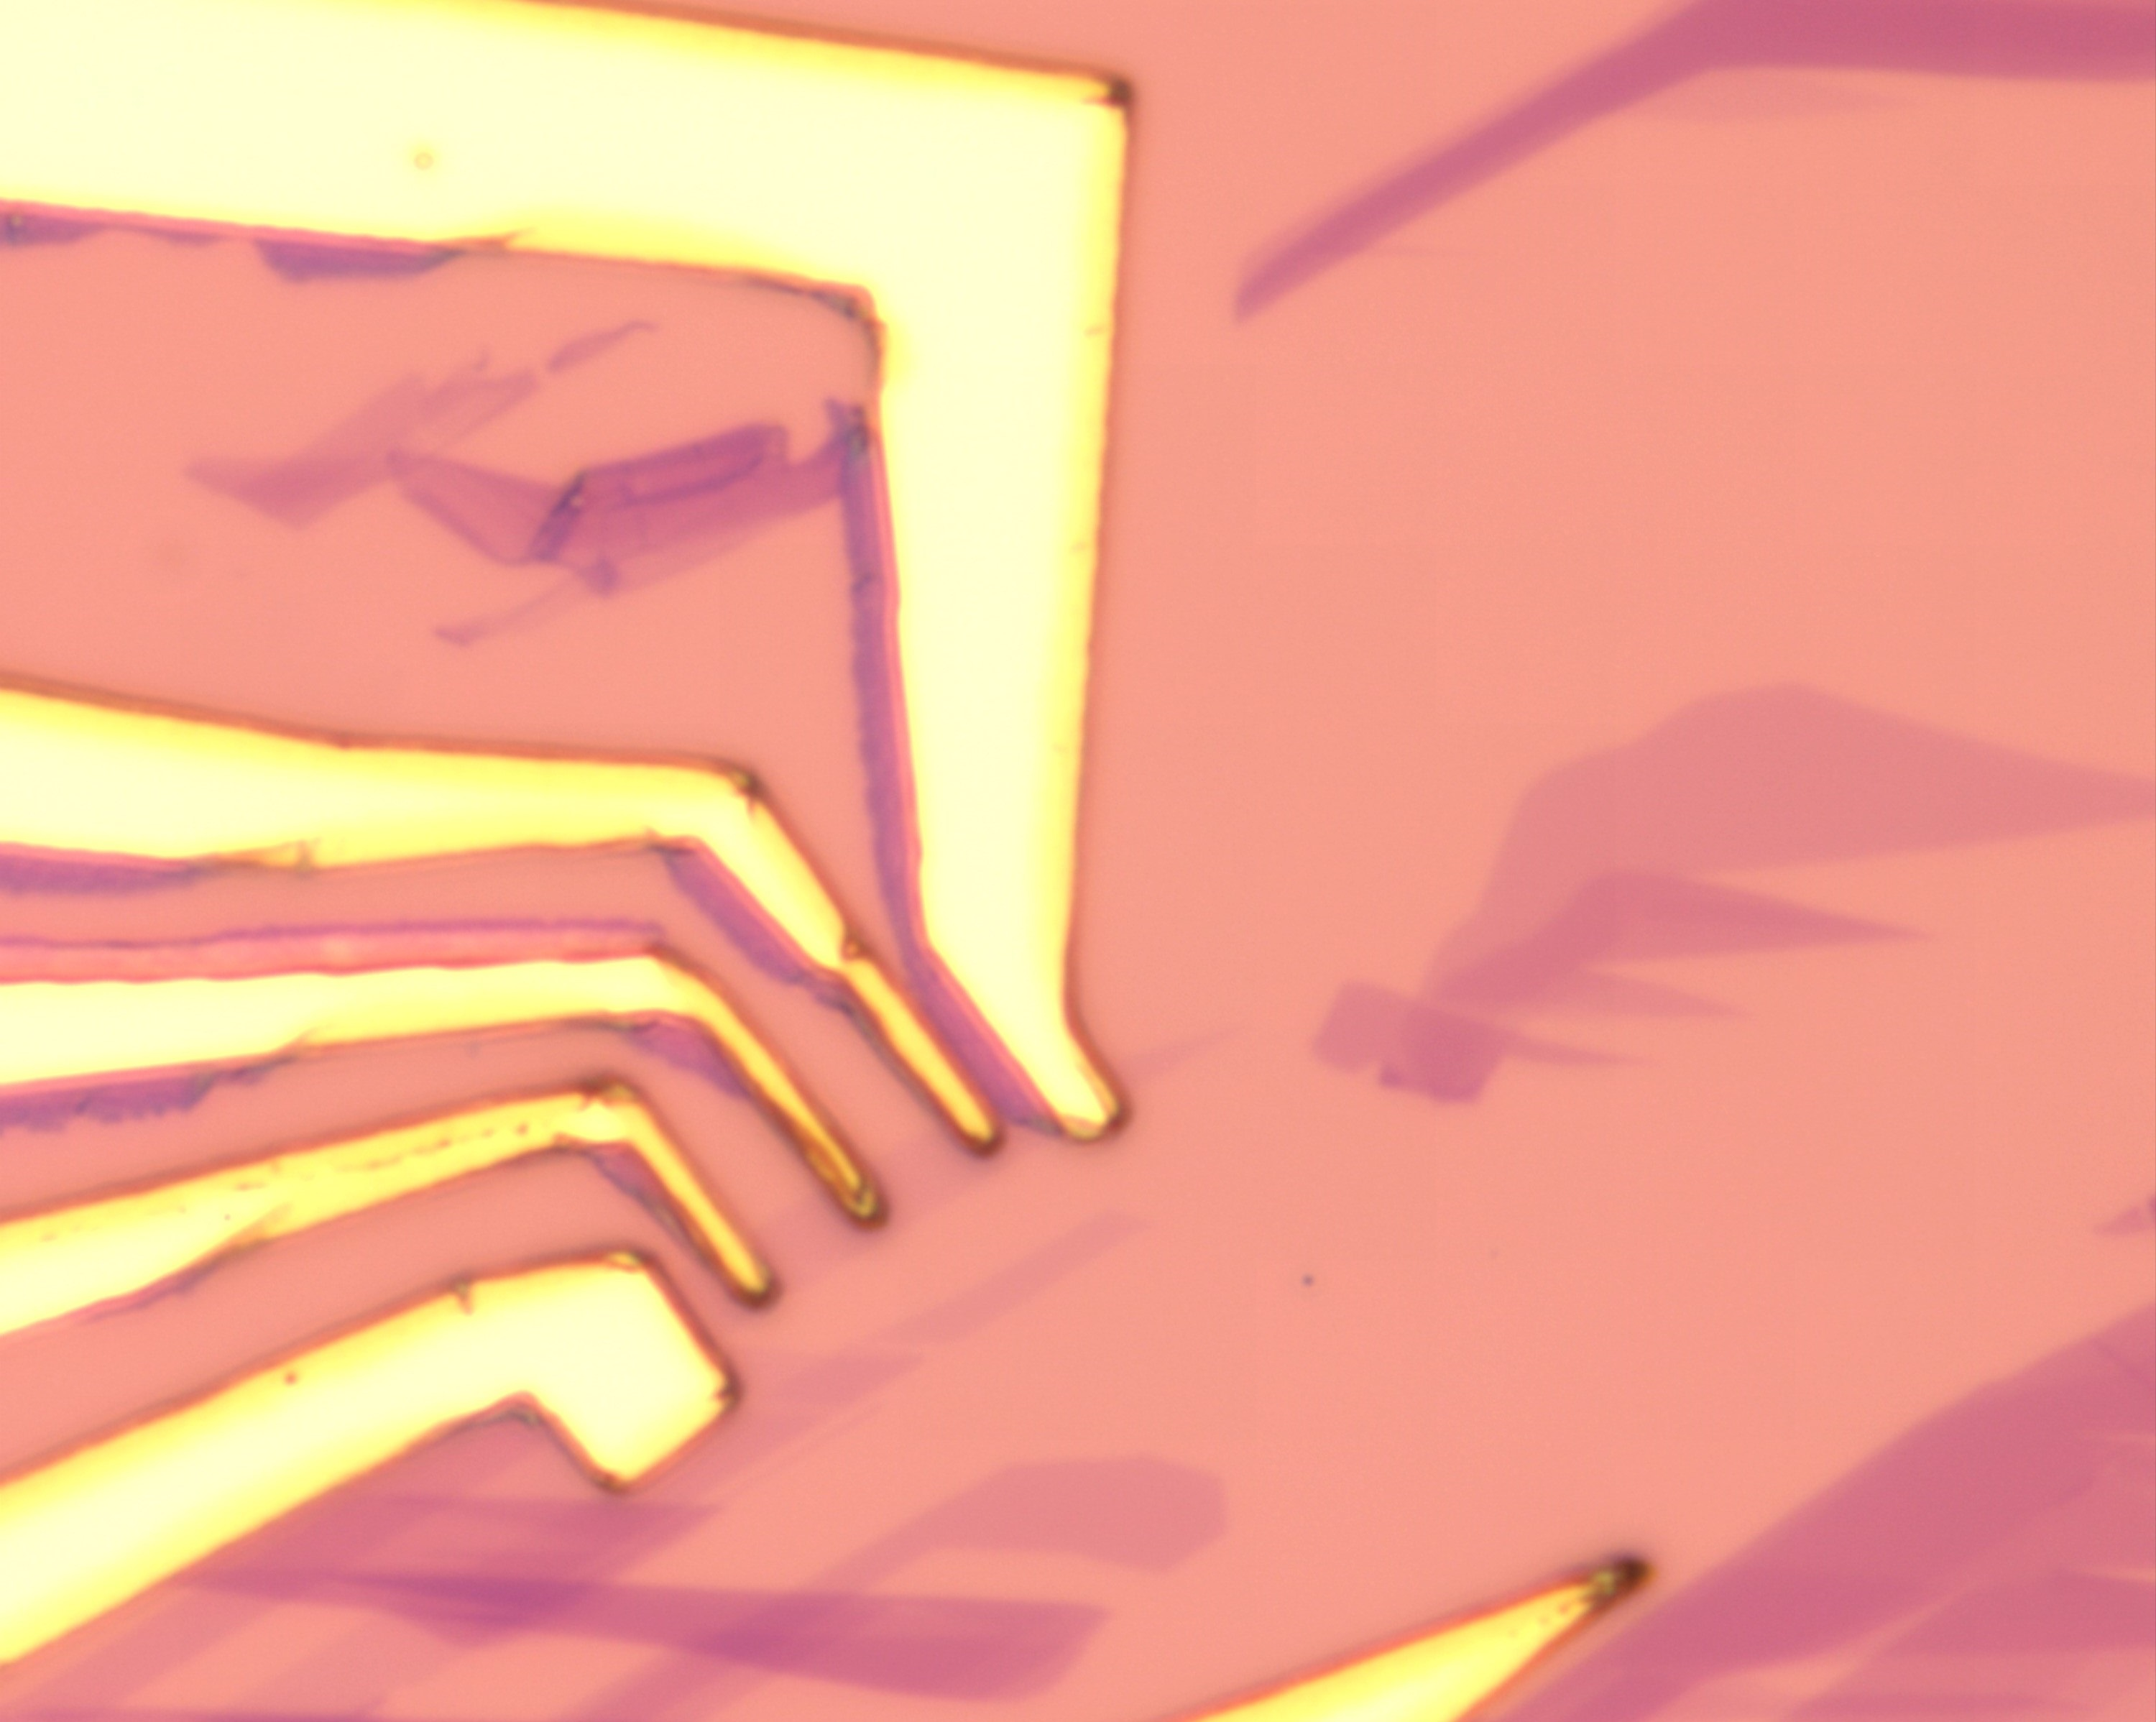
\includegraphics[width=\textwidth]{chap2/skins/2_100x_v2.jpg}
%			\subcaption{after 10s ultrasonication}		
		\end{subfigure}
		\caption[Material remanants from lithography]{Material remanants from lithography. Gold edges exhibit a bluish remnant edge.}\label{fig:lithography_skins}
	\end{figure}
	
	This is likely due to metal deposition (ie, Chromium, see \cref{sec:deposition}) forming layers on the sides of lithography wells, as the skins have very similar geometry to that of either the wells or the edges. The spinning speeds give resist heights (ie, the well edge heights) roughly the same as feature width ($\approx$1$\mu$m minimum), matching the observed result. 
	
	Ultrasonication (see \cref{sec:ultrasonication}) can be used to attempt to remove edges after lift off, however there is risk of damaging samples of graphene.
	
	\paragraph{LOR-1A \& AZ-1512HS}
	The issue with a single layer photoresist processes, outlined above, is that well edges allow deposited materials to adhere, leaving 'skins'. One way to prevent this from happening is to use a multilayer process. Two resist layers are spun onto the sample, with the bottom film being more sensitive to the lithography process than the top (ie, develops faster, or is more sensitive to exposure). When developed, the bottom layer \textit{undercuts} the top layer, stopping adhesion to edges of the well when material is deposited. This process is depicted in \cref{fig:bilayer_lithography}.
	
	\begin{figure}[H]
		\centering
		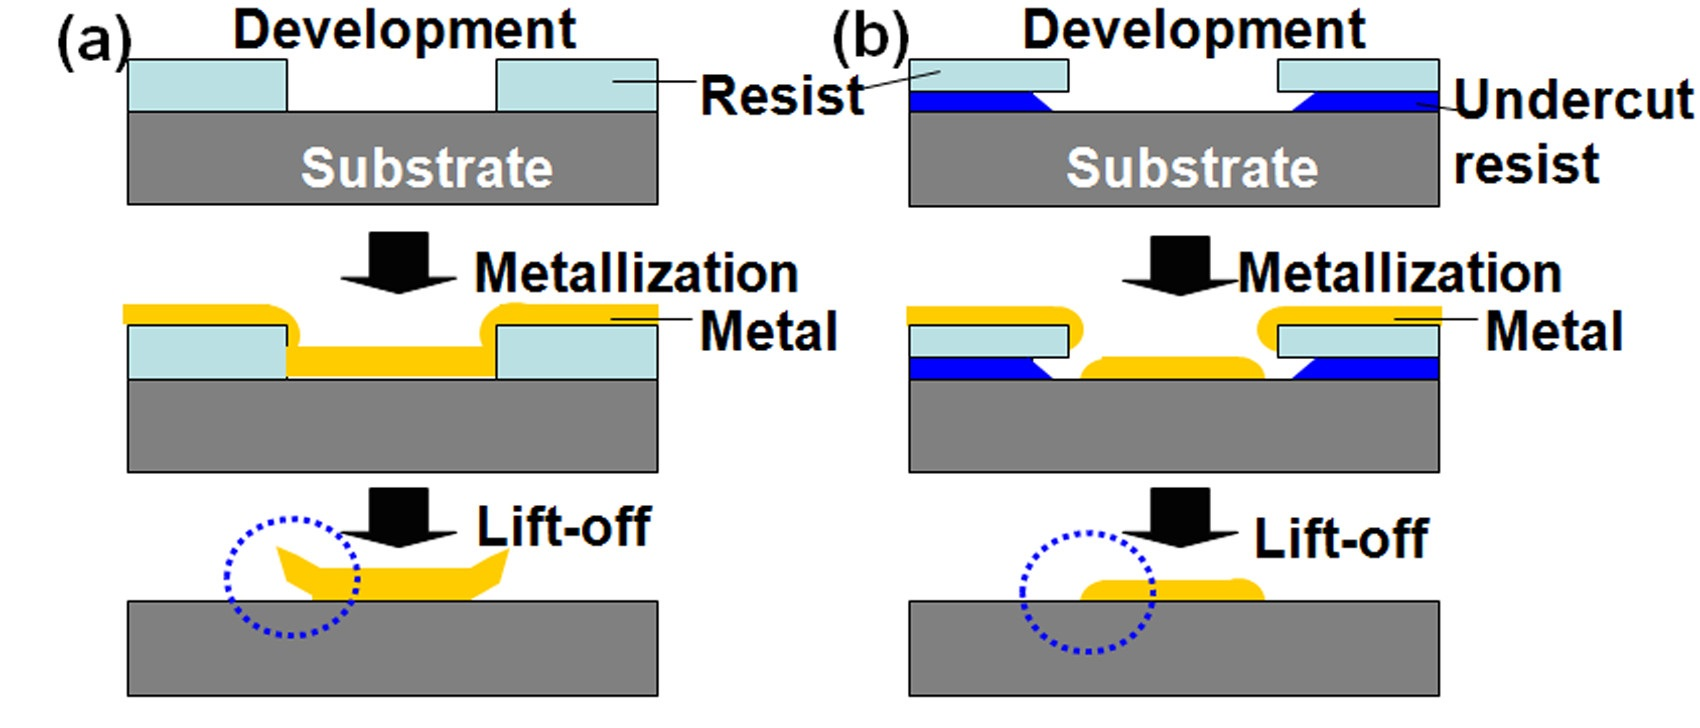
\includegraphics[width=0.5\textwidth]{chap2/bilayerResist.jpeg}
		\caption[Bilayer lithography process]{Bilayer lithography process (Source: Park \etal\cite{park_bilayer_2008}) }\label{fig:bilayer_lithography}
	\end{figure}
	
	LOR-1A is an actinic lift off resist, responding to UV light from 240 nm to 290 nm \cite{microchem_lor1a}. When the resist films are exposed to the developer, LOR-1A is removed below an overhanging AZ1512-HS layer due to additional development, leaving the desired undercut effect.
	
	\subsubsection{Exposure}\label{sec:exposure}
	After spinning, a mask writer tool is used to expose the wafer and resist films to UV light. A mask writer is composed of a mask, or a DMD (digital micro-mirror device) which allows filtering of pixel like squares, based on an imput image. Actinic reactions occur from the UV light with the photoresist, forming desired pad structures in the resist. Prepared CAD files are used to generate masks used by the DMD as seen in \cref{fig:DMD_mask}.
	
	\begin{figure}
		\centering
		\begin{subfigure}{0.65\textwidth}
			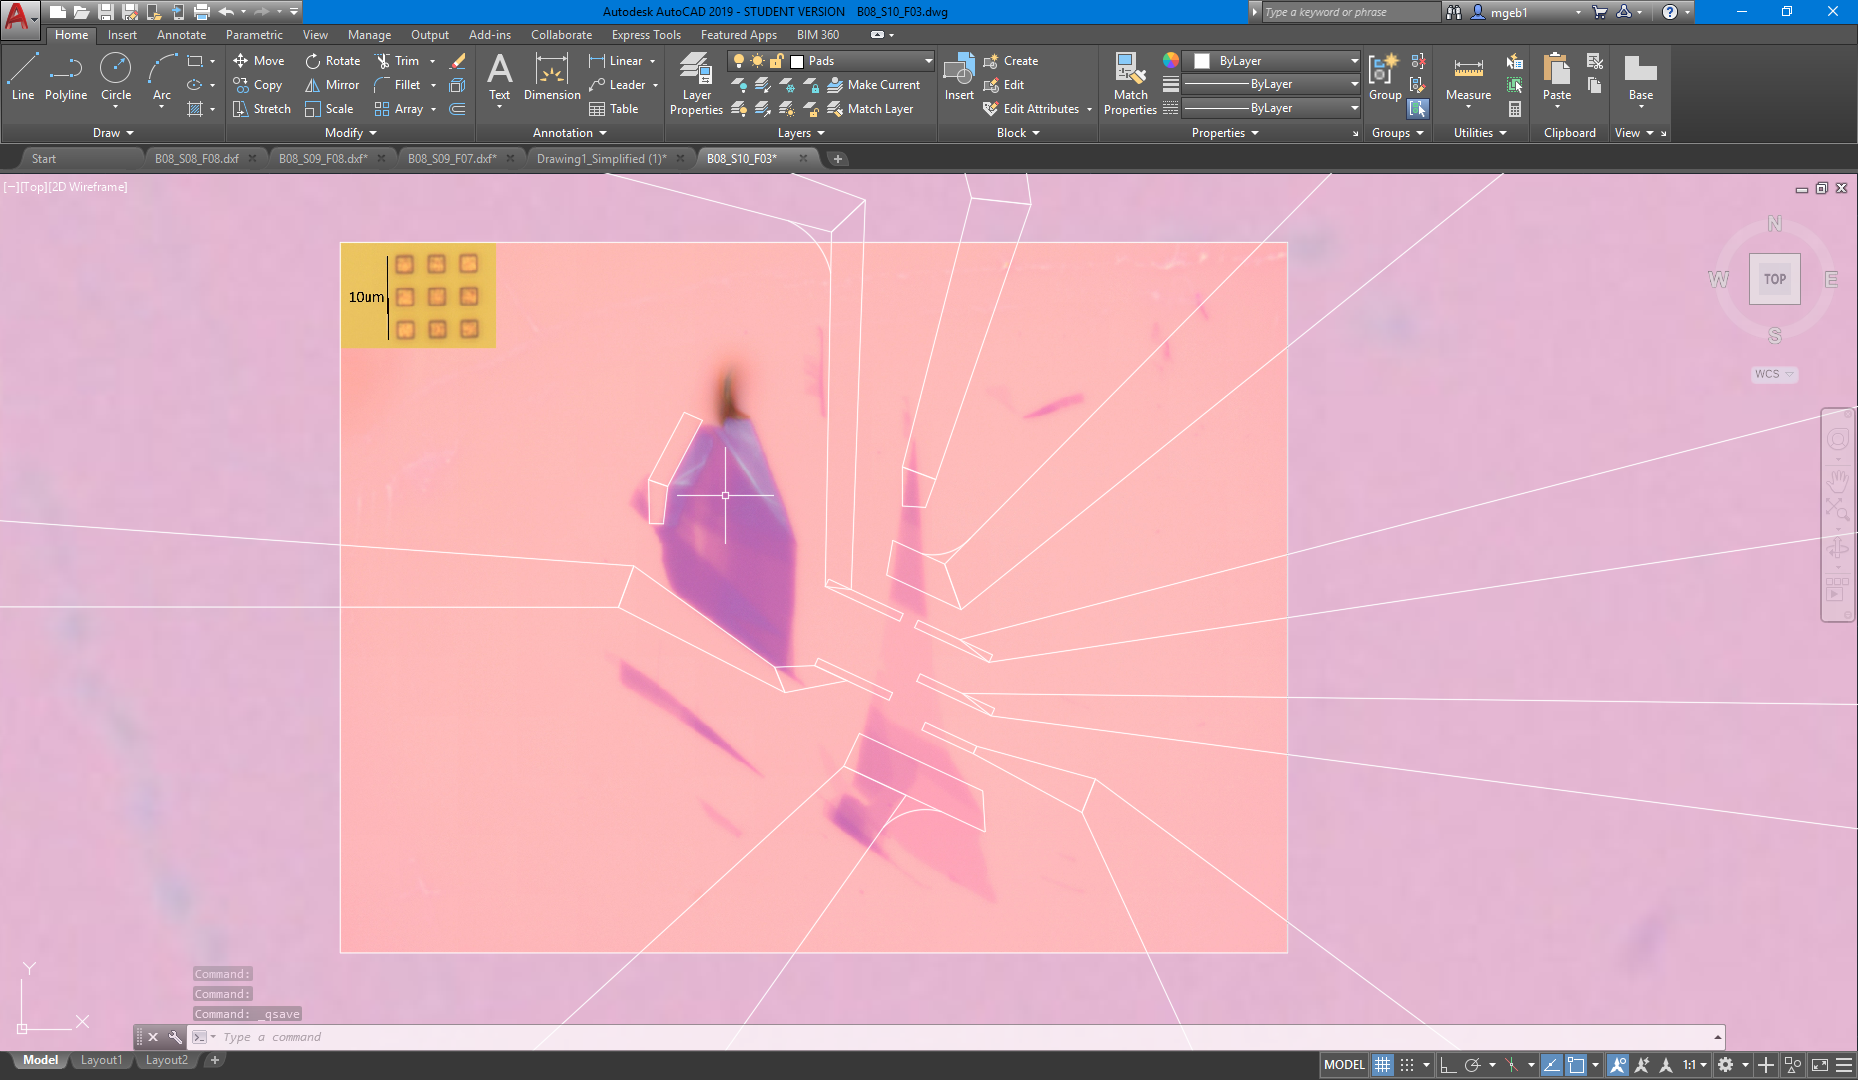
\includegraphics[width=\textwidth]{chap2/DMD_mask}
			\caption[DMD masks created using Autocad\texttrademark.]{DMD masks created using Autocad\texttrademark. Additional structures are created to help position the mask when using a 20x lens, as graphene can be difficult to see in a mask writer tool.}
		\end{subfigure}
		\hspace{0.02\textwidth}
		\begin{subfigure}{0.3\textwidth}
			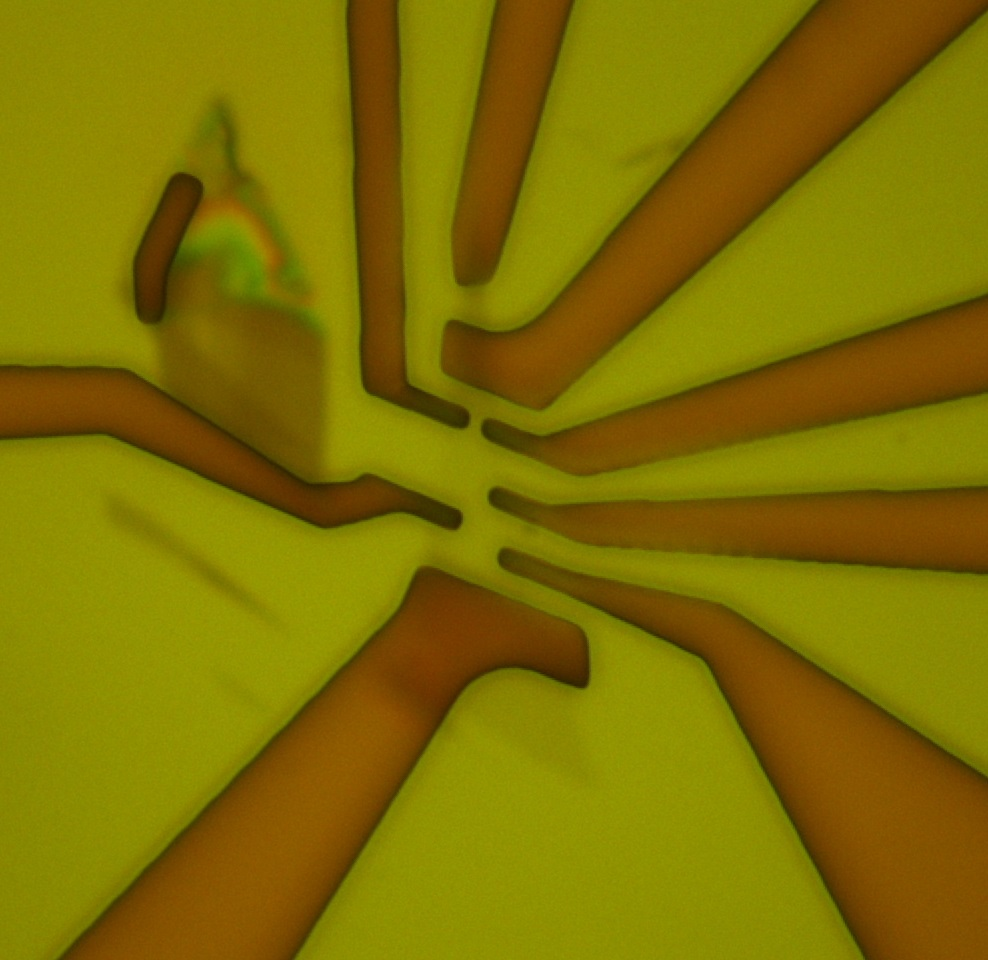
\includegraphics[width=\textwidth]{chap2/mask}
			\caption[Photolithography structure]{Photolithography structure from mask writing and development.}
		\end{subfigure}
		\caption{Photolithography mask writing}\label{fig:DMD_mask}
	\end{figure}
	
	An important parameter in the mask writing process is the exposure time, which affects the ability to develop fine structures. By using an array of different exposure times (\cref{fig:exposure_array}), the optimal feature result was found for a typical developing time.
	
	\begin{figure}[H]
		\centering
		\begin{subfigure}{0.45\textwidth}
			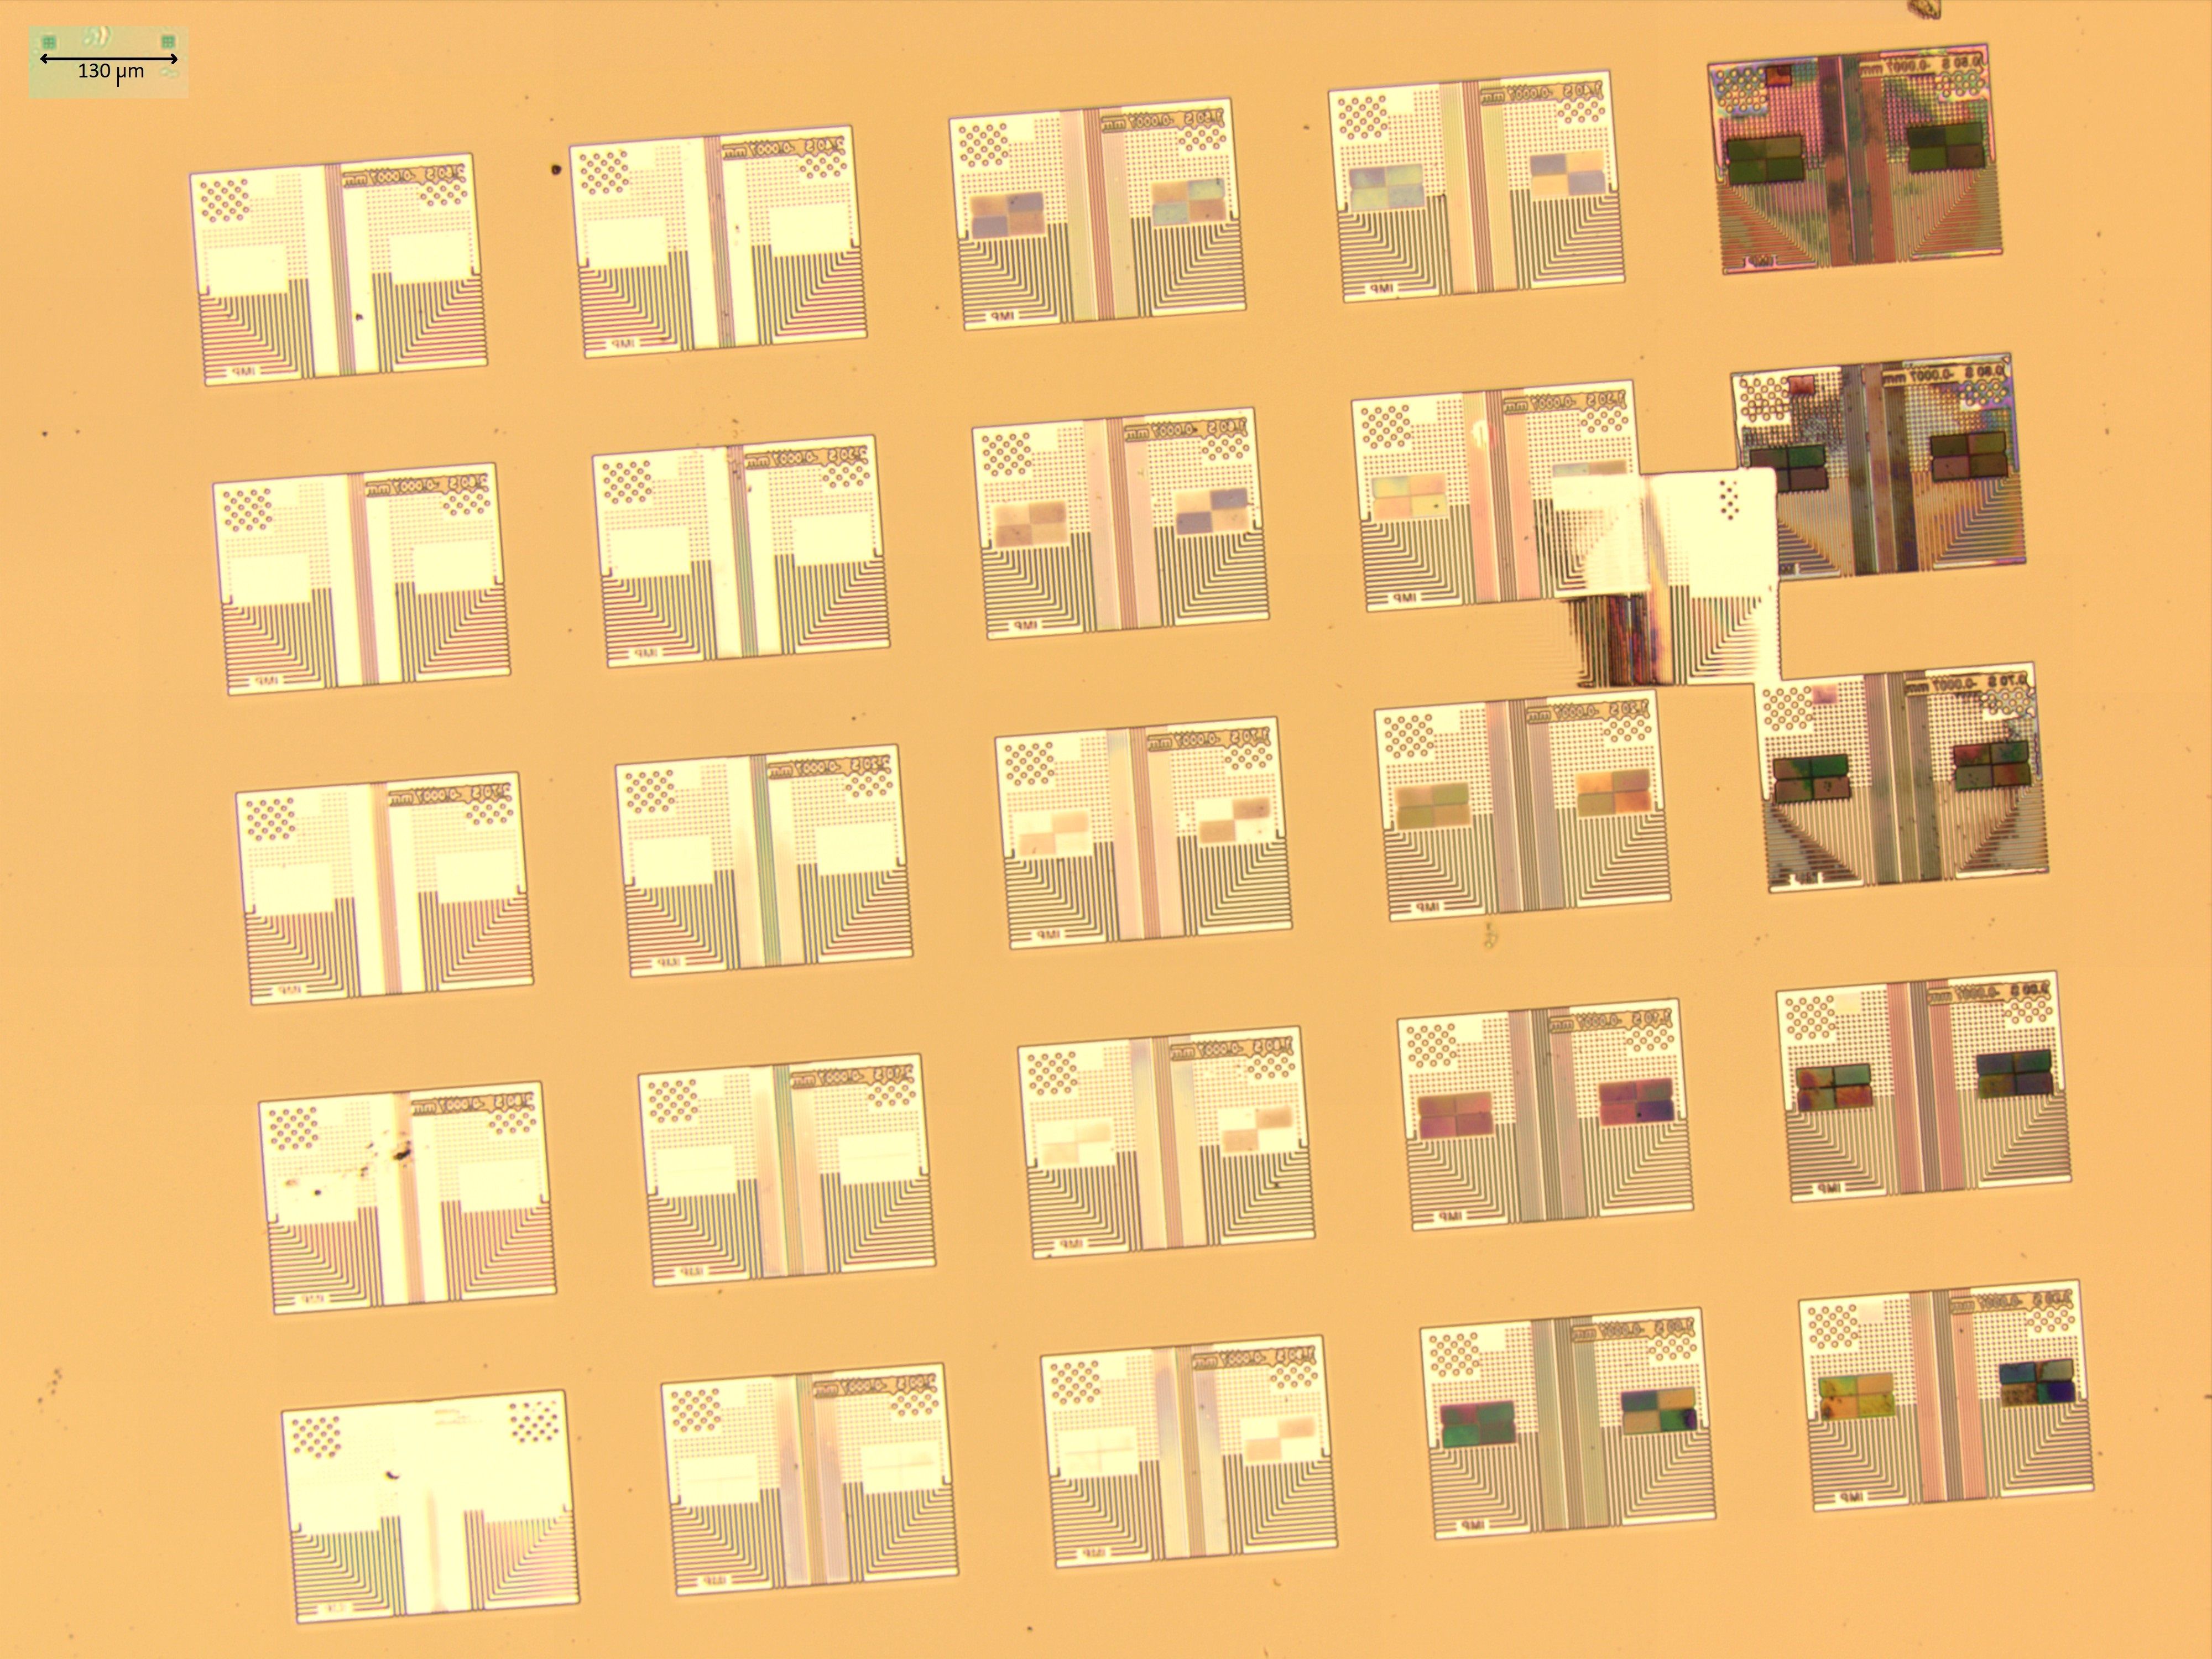
\includegraphics[width=\textwidth]{chap2/array/array1}
			\caption{Feature array 5x}
		\end{subfigure}
		\begin{subfigure}{0.45\textwidth}
			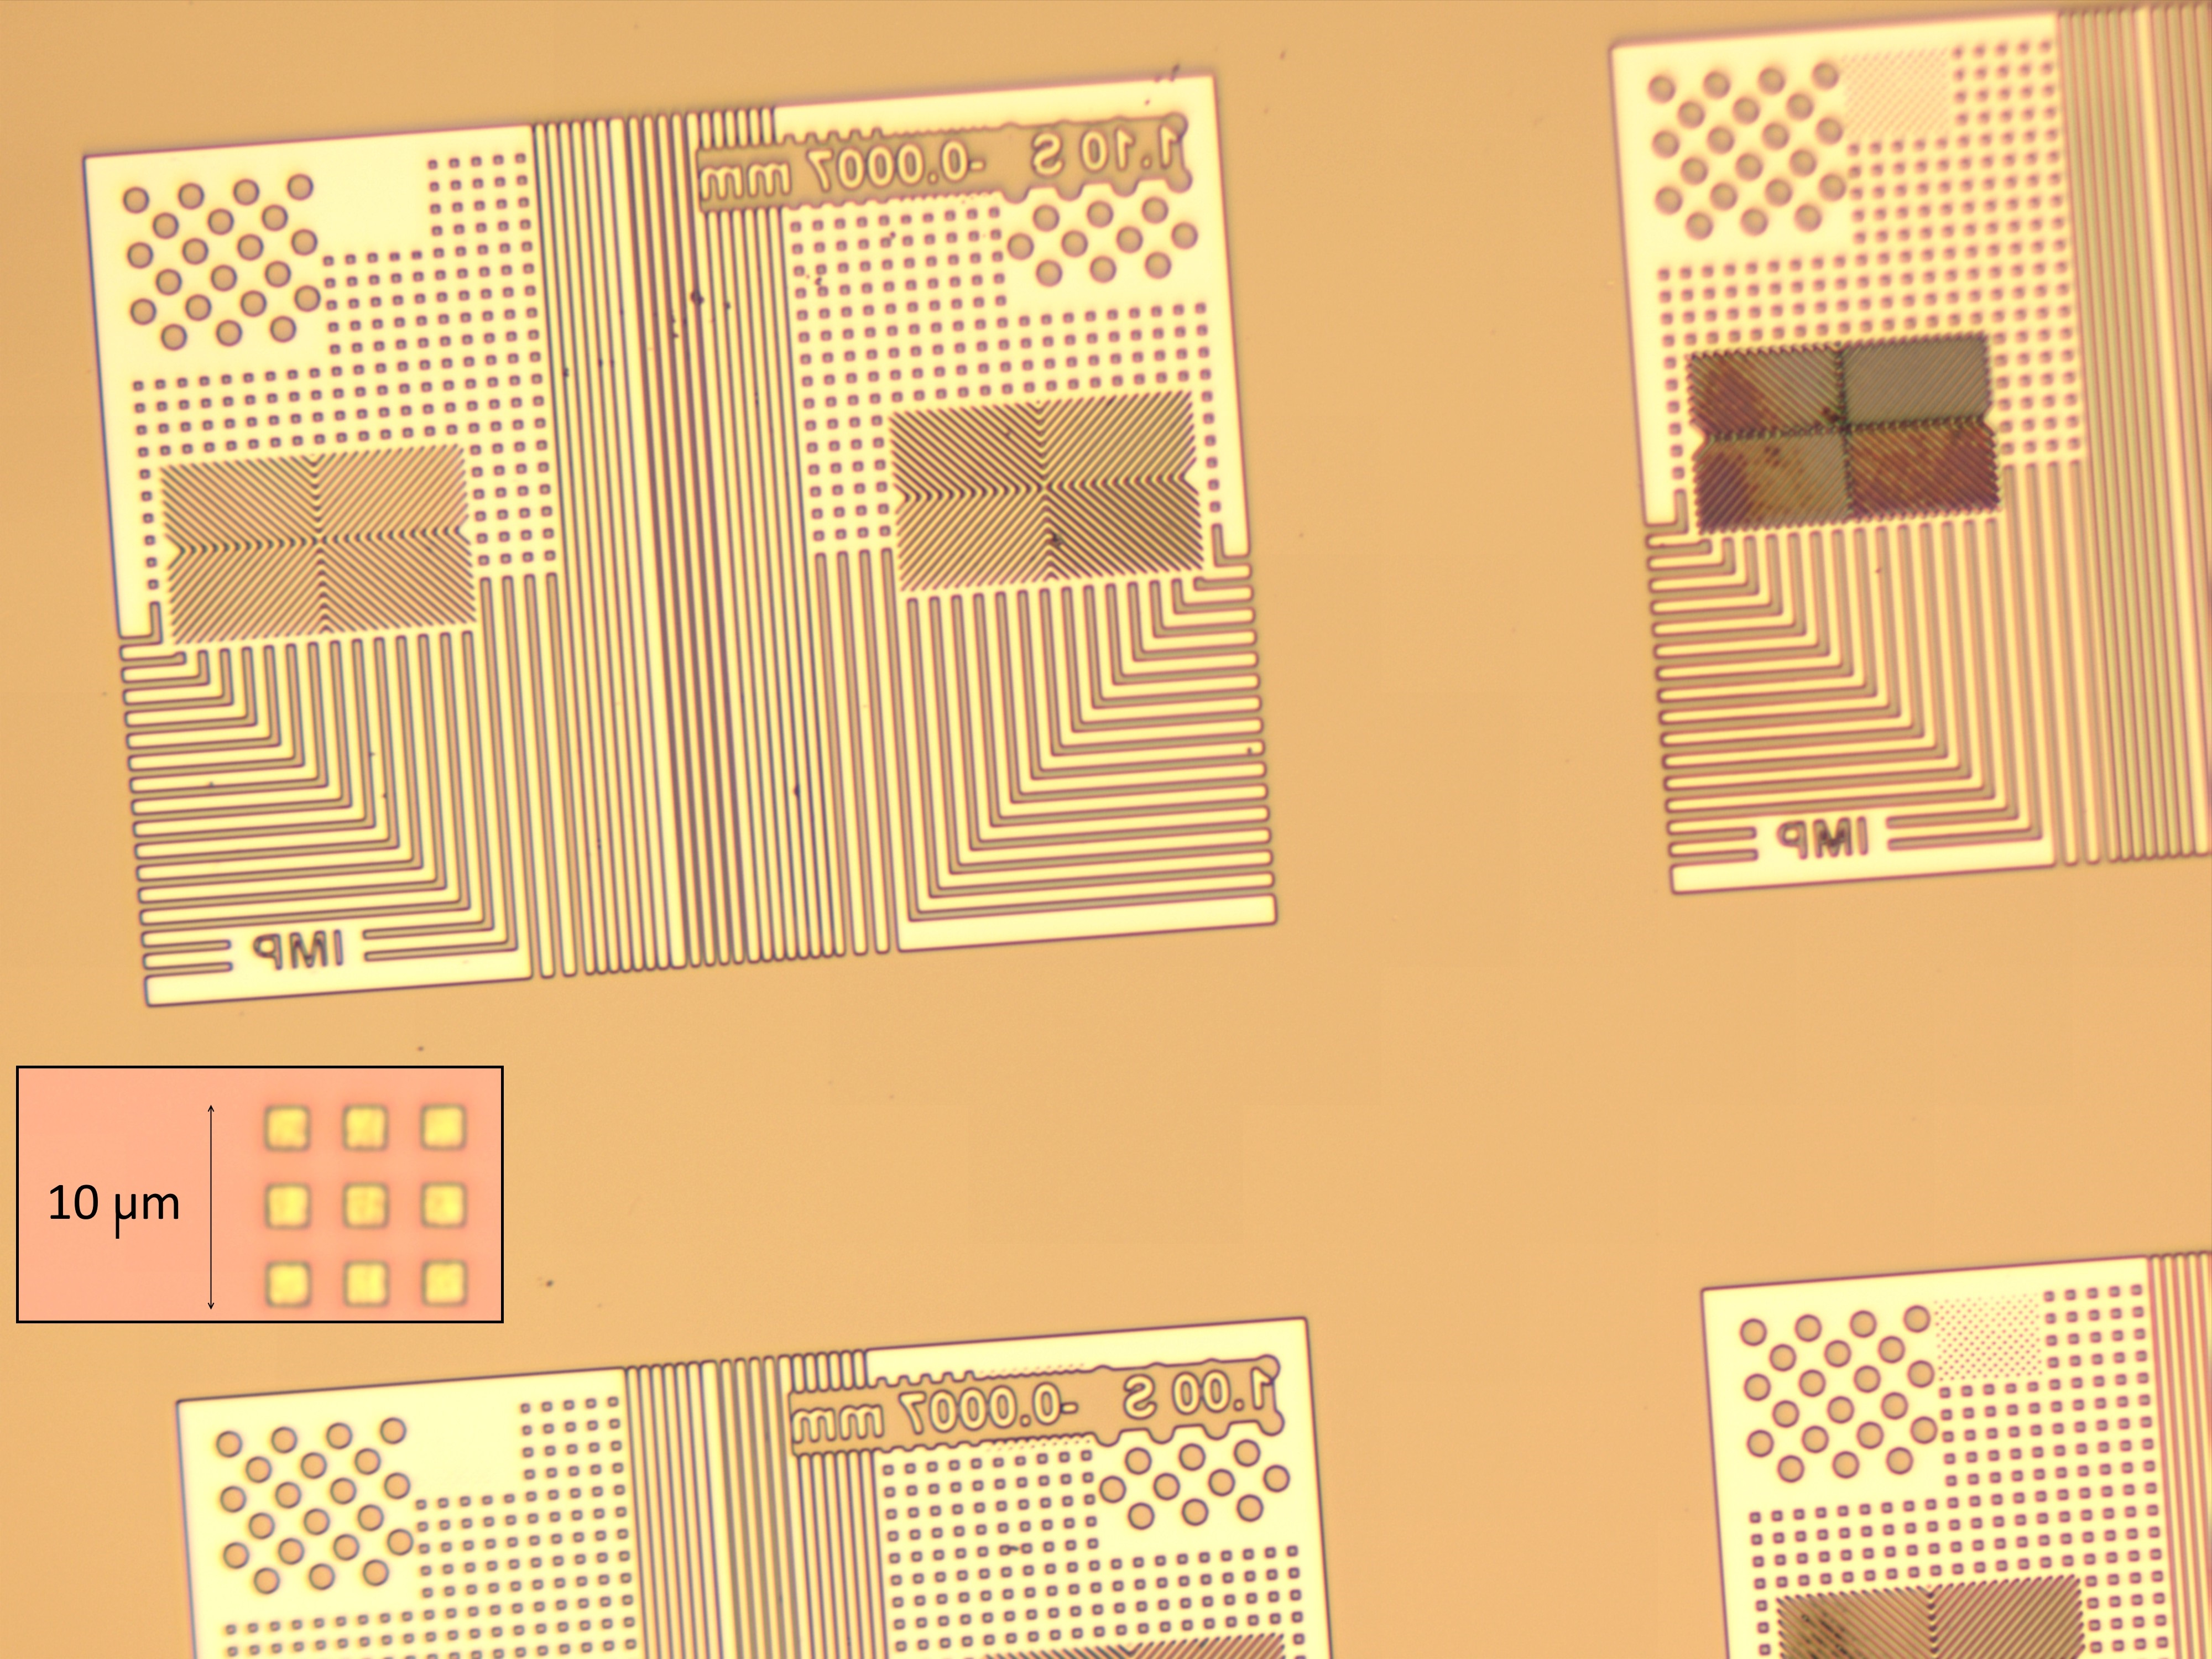
\includegraphics[width=\textwidth]{chap2/array/array2}
			\caption{Feature array 100x}
		\end{subfigure}
		\caption{Developing an exposure array on \silicondioxide}\label{fig:exposure_array}
	\end{figure}
	
	\subsubsection{Developers}\label{sec:developer}
	Developers are used to dissolve exposed / unexposed areas of photoresist films. We use AZ-726 in conjunction with AZ-1512HS. Using a development time complementary to the exposure time is important to not overdevelop features, as material in proximity to exposed areas is at risk of some structural damage, and developers continue to react with the remaining structure over time.
	
	\subsection{UV Ozone surface preparation}\label{sec:uv_ozone}
	%TODO Cite papers here.
	Large resistances can occur when trying to make contact with graphene. This can be for a variety of reasons. Resist residues between the deposited pads and graphene can be insulating, perhaps non-metalic bonding occurs between deposited metals and graphene, or the oxidisation of metals being deposited (ie, chromium oxide) could occur.
	
	Serveral studies by Li \etal\cite{li_ultraviolet/ozone_2013} and Nath \etal\cite{nath_achieving_2014,nath_search_2016} have shown the ability to reduce contact resistance of graphene by using UV ozone treatement, to less than 200 $\Omega$, a small contact resistance.
	
	\begin{figure}[H]
		\centering
		\includegraphics[width=0.6\textwidth]{chap2/uvozone/UVOzone}
		\caption{Cleaning of graphene using UV Ozone (Source: Li \etal. \cite{li_ultraviolet/ozone_2013})}\label{fig:UV_ozone} (a) Before transfer (b) After photolithography  (c)$\to$(f) UVO treatment for 5, 10, 16, 22 min, respectively. Scale bar: 1$\mu$m.
	\end{figure}
	
	UV Ozone treatment refers to the use of UV light to generate photochemical reactions on sample surfaces. $185$nm light is used to generate ozone O$_3$ from bonding molecular (O$_2$) oxygen, while $254$nm light is used to dissociate ozone to molecular and singlet oxygen (O$_1$), the latter of which is reactive with substrate surfaces. Increasing stage temperature also will increase the etching rate that occurs. UV Ozone is used in this context to clean the graphene exposed in our developed wells, as seen in \cref{fig:UV_ozone}.
	
	\begin{wrapfigure}[13]{r}[0pt]{5.5cm}
		\vspace{-0.5cm}
		\centering
		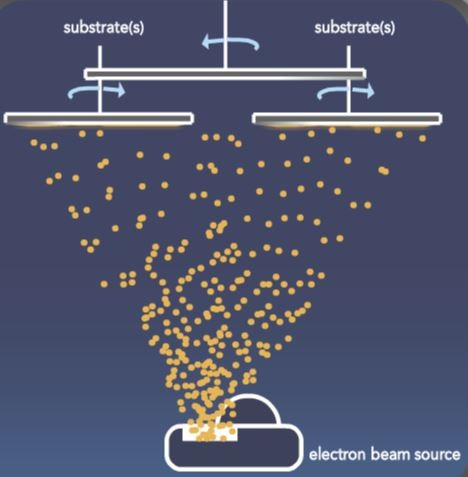
\includegraphics[width=0.32\textwidth]{chap2/deposition}
		\caption{E-beam Evaporation (Source: \cite{noauthor_understanding_nodate})}\label{fig:ebeamevap}
	\end{wrapfigure}
	
	To determine an appropriate etching time for the particular tool used, two wafers with grapehe flakes at times of 5m and 15m were cleaned using UV Ozone. The 15m devices were etched away completely, however the 5m device provided the first low resistance contact observed, after many iterations of devices.
	
	
	\subsection{Deposition}\label{sec:deposition}

	Once a designed structure is built to make contacts with graphene and cleaned using UV Ozone, material can now be deposited onto the device. There are many different methods, including sputtering and thermal evaporation, however electron beam evaporation (\cref{fig:ebeamevap}) was used for these devices, due to its uniformity, control of deposition rate, and the availability of various material crucibles.
	
	50nm of Au (Gold) was originally deposited with a Cr (Chromium) adhesion layer of 5nm to promote contact to SiO$_2$, however issues with metallic contact to graphene arose. In case of chromium oxidisation during deposition, creating an insulating layer to graphene, a thinner layer (2nm) of chromium was instead deposited. This is reasonable as pinhole effects resulting from a thin deposited Cr layer do not affect bulk transport.
	
	\subsubsection{Oxide Protection}\label{sec:deposition_oxide_protection}
	
	\begin{wrapfigure}[13]{r}[0pt]{5.5cm}
		\vspace{-1cm}
		\centering
		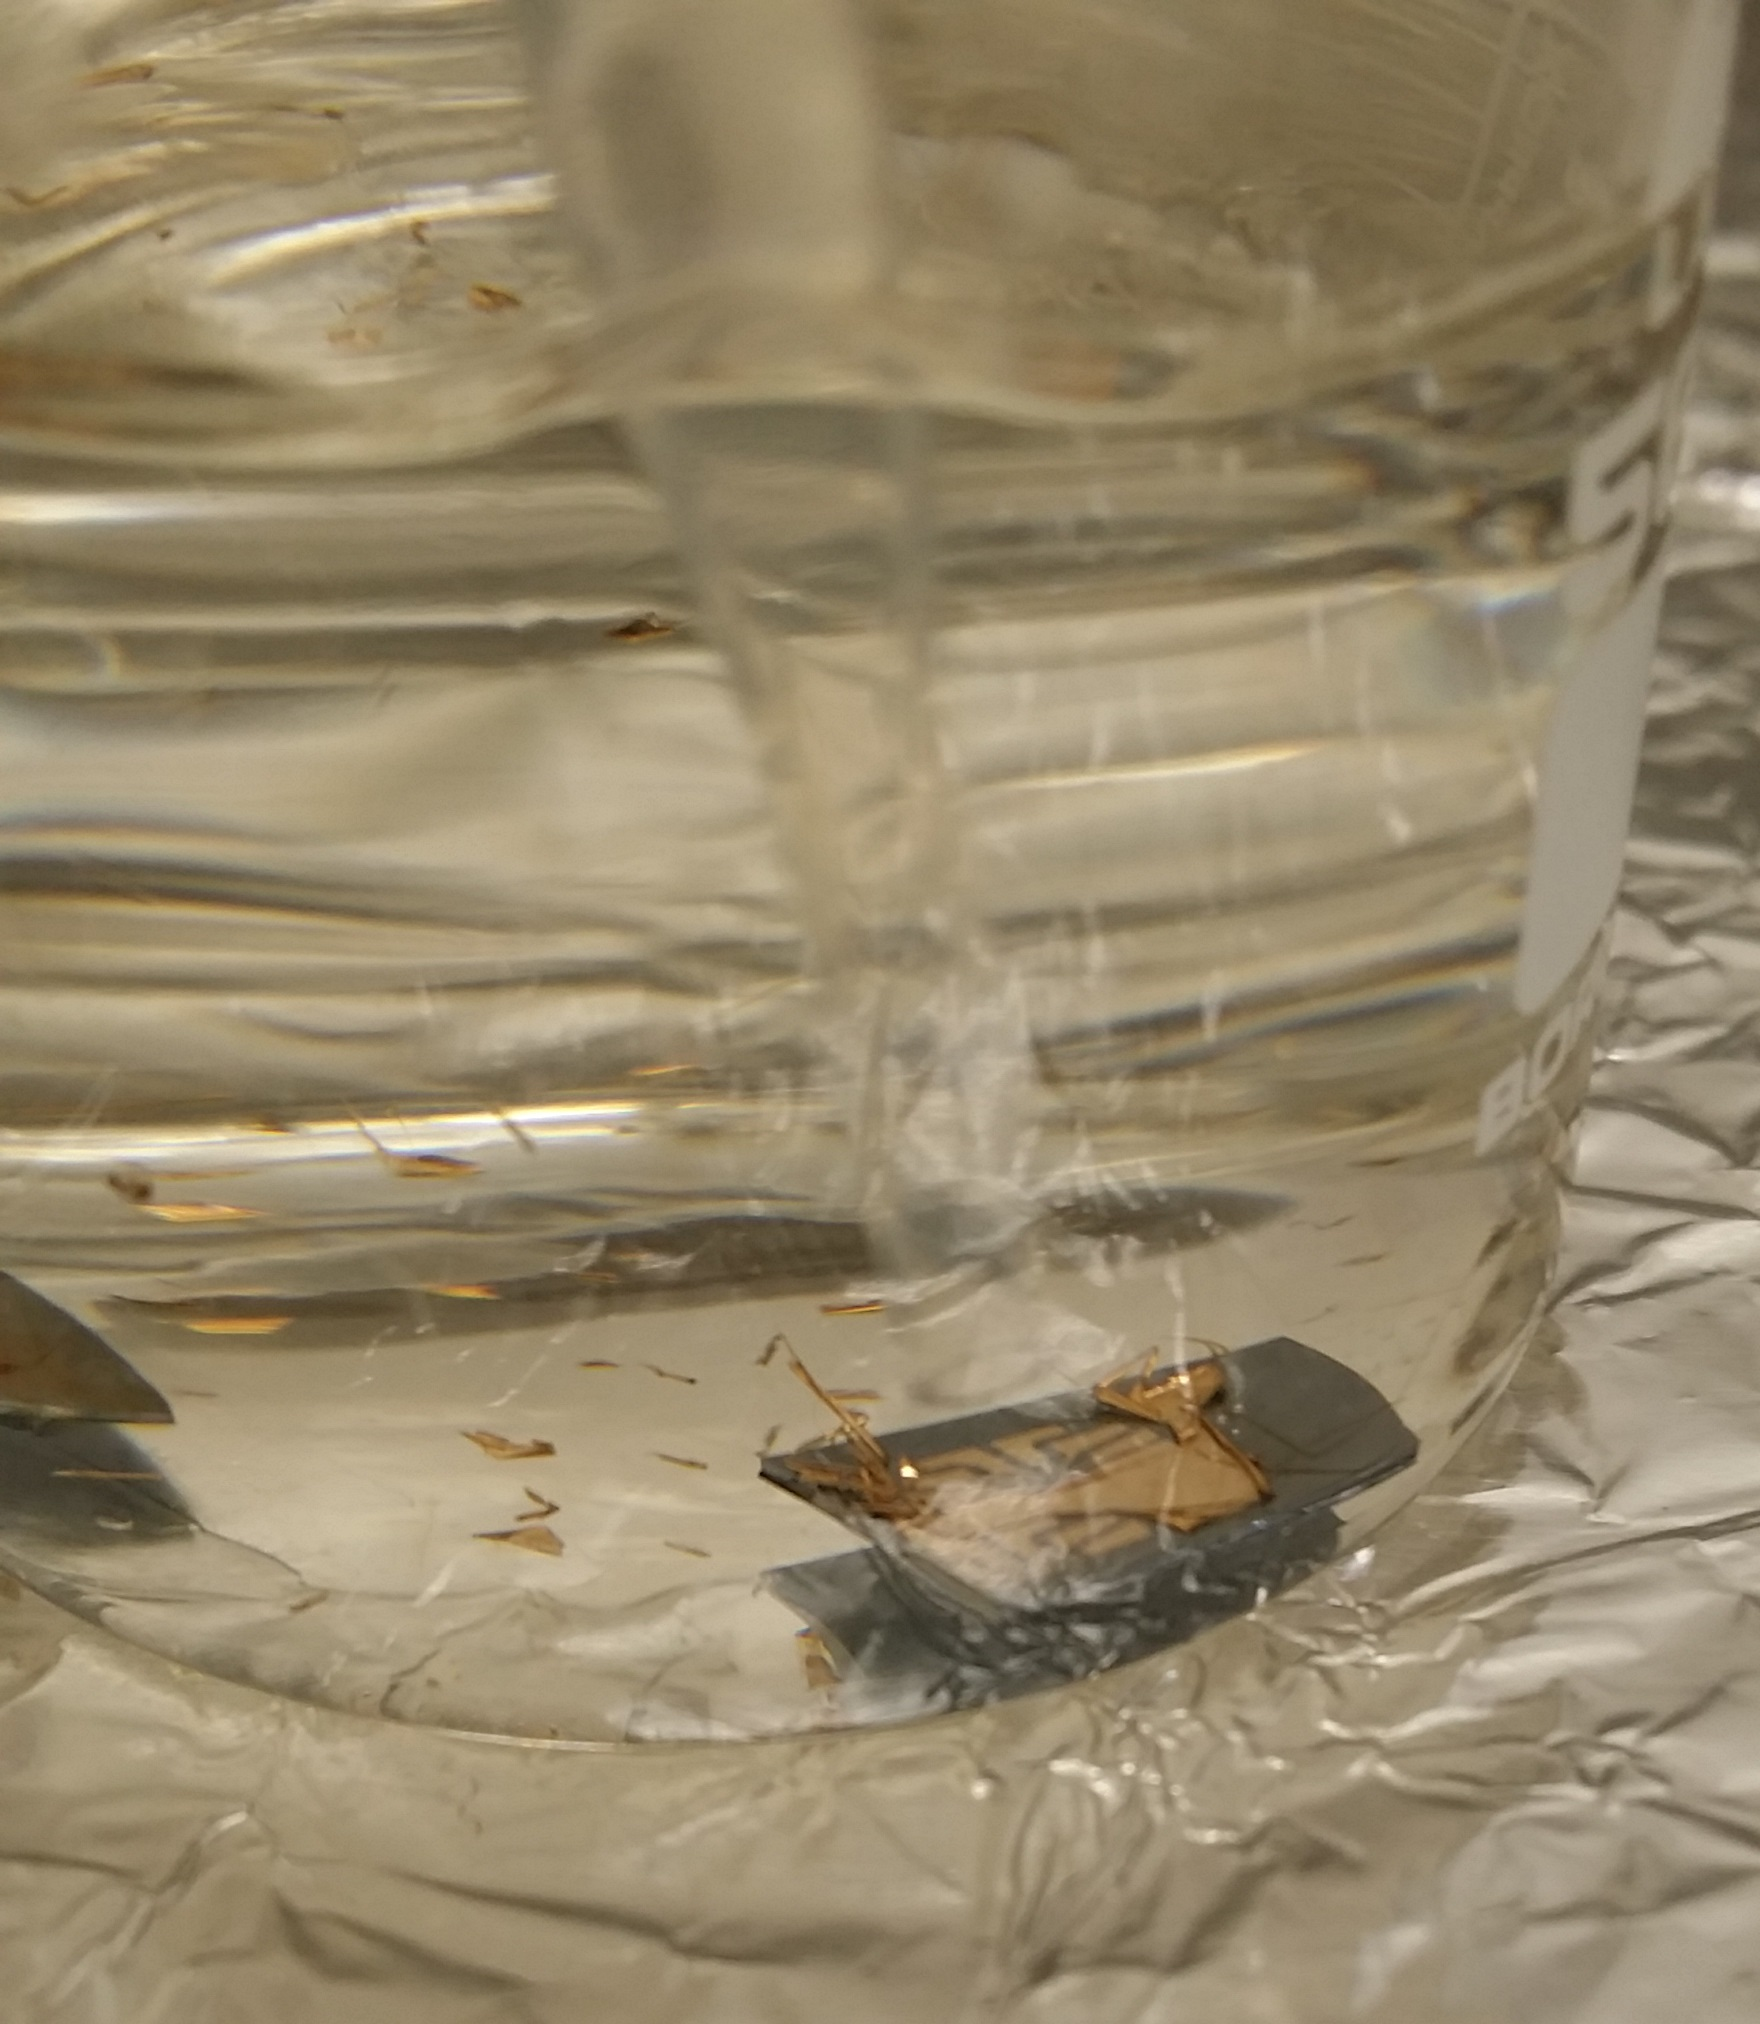
\includegraphics[width=0.32\textwidth]{chap2/liftoff}
		\caption{PG Remover liftoff}\label{fig:liftoff}
	\end{wrapfigure}

	In using metal liquids to cover devices with oxides, the gold reacted strongly to the liquid metallic environment, destroying pre-established pads. This is further described in \cref{chap:thinoxides}, however the result was to use additional layers, another layer of Cr 2nm and a layer of SiO$_2$ 20nm. These additional layers do not prevent contact through contact probes and provide insulation from the bulk of metal liquid reactions.
	
	\subsection{Lift-off}\label{sec:liftoff}
	To remove the remaining gold covered photoresist on the substrate, a solvent called PG remover is used to emerse samples at 80 $^\circ$C. Using a pipette to generate soft fluid flow around the device, the excess gold is slowly removed. 
	
	\subsubsection{Ultrasonication}\label{sec:ultrasonication}
	After lift off, the presence of skin remenants (described in \cref{sec:skin_issues}) could sometimes be cleaned off through the use of ultrasonication (\cref{fig:lithography_skins_us}), however this had a large risk of damaging the graphene, seen in \cref{fig:lithography_skins_break}.
	
	\begin{figure}[H]
		\centering
		\begin{subfigure}[b]{0.3\textwidth}
			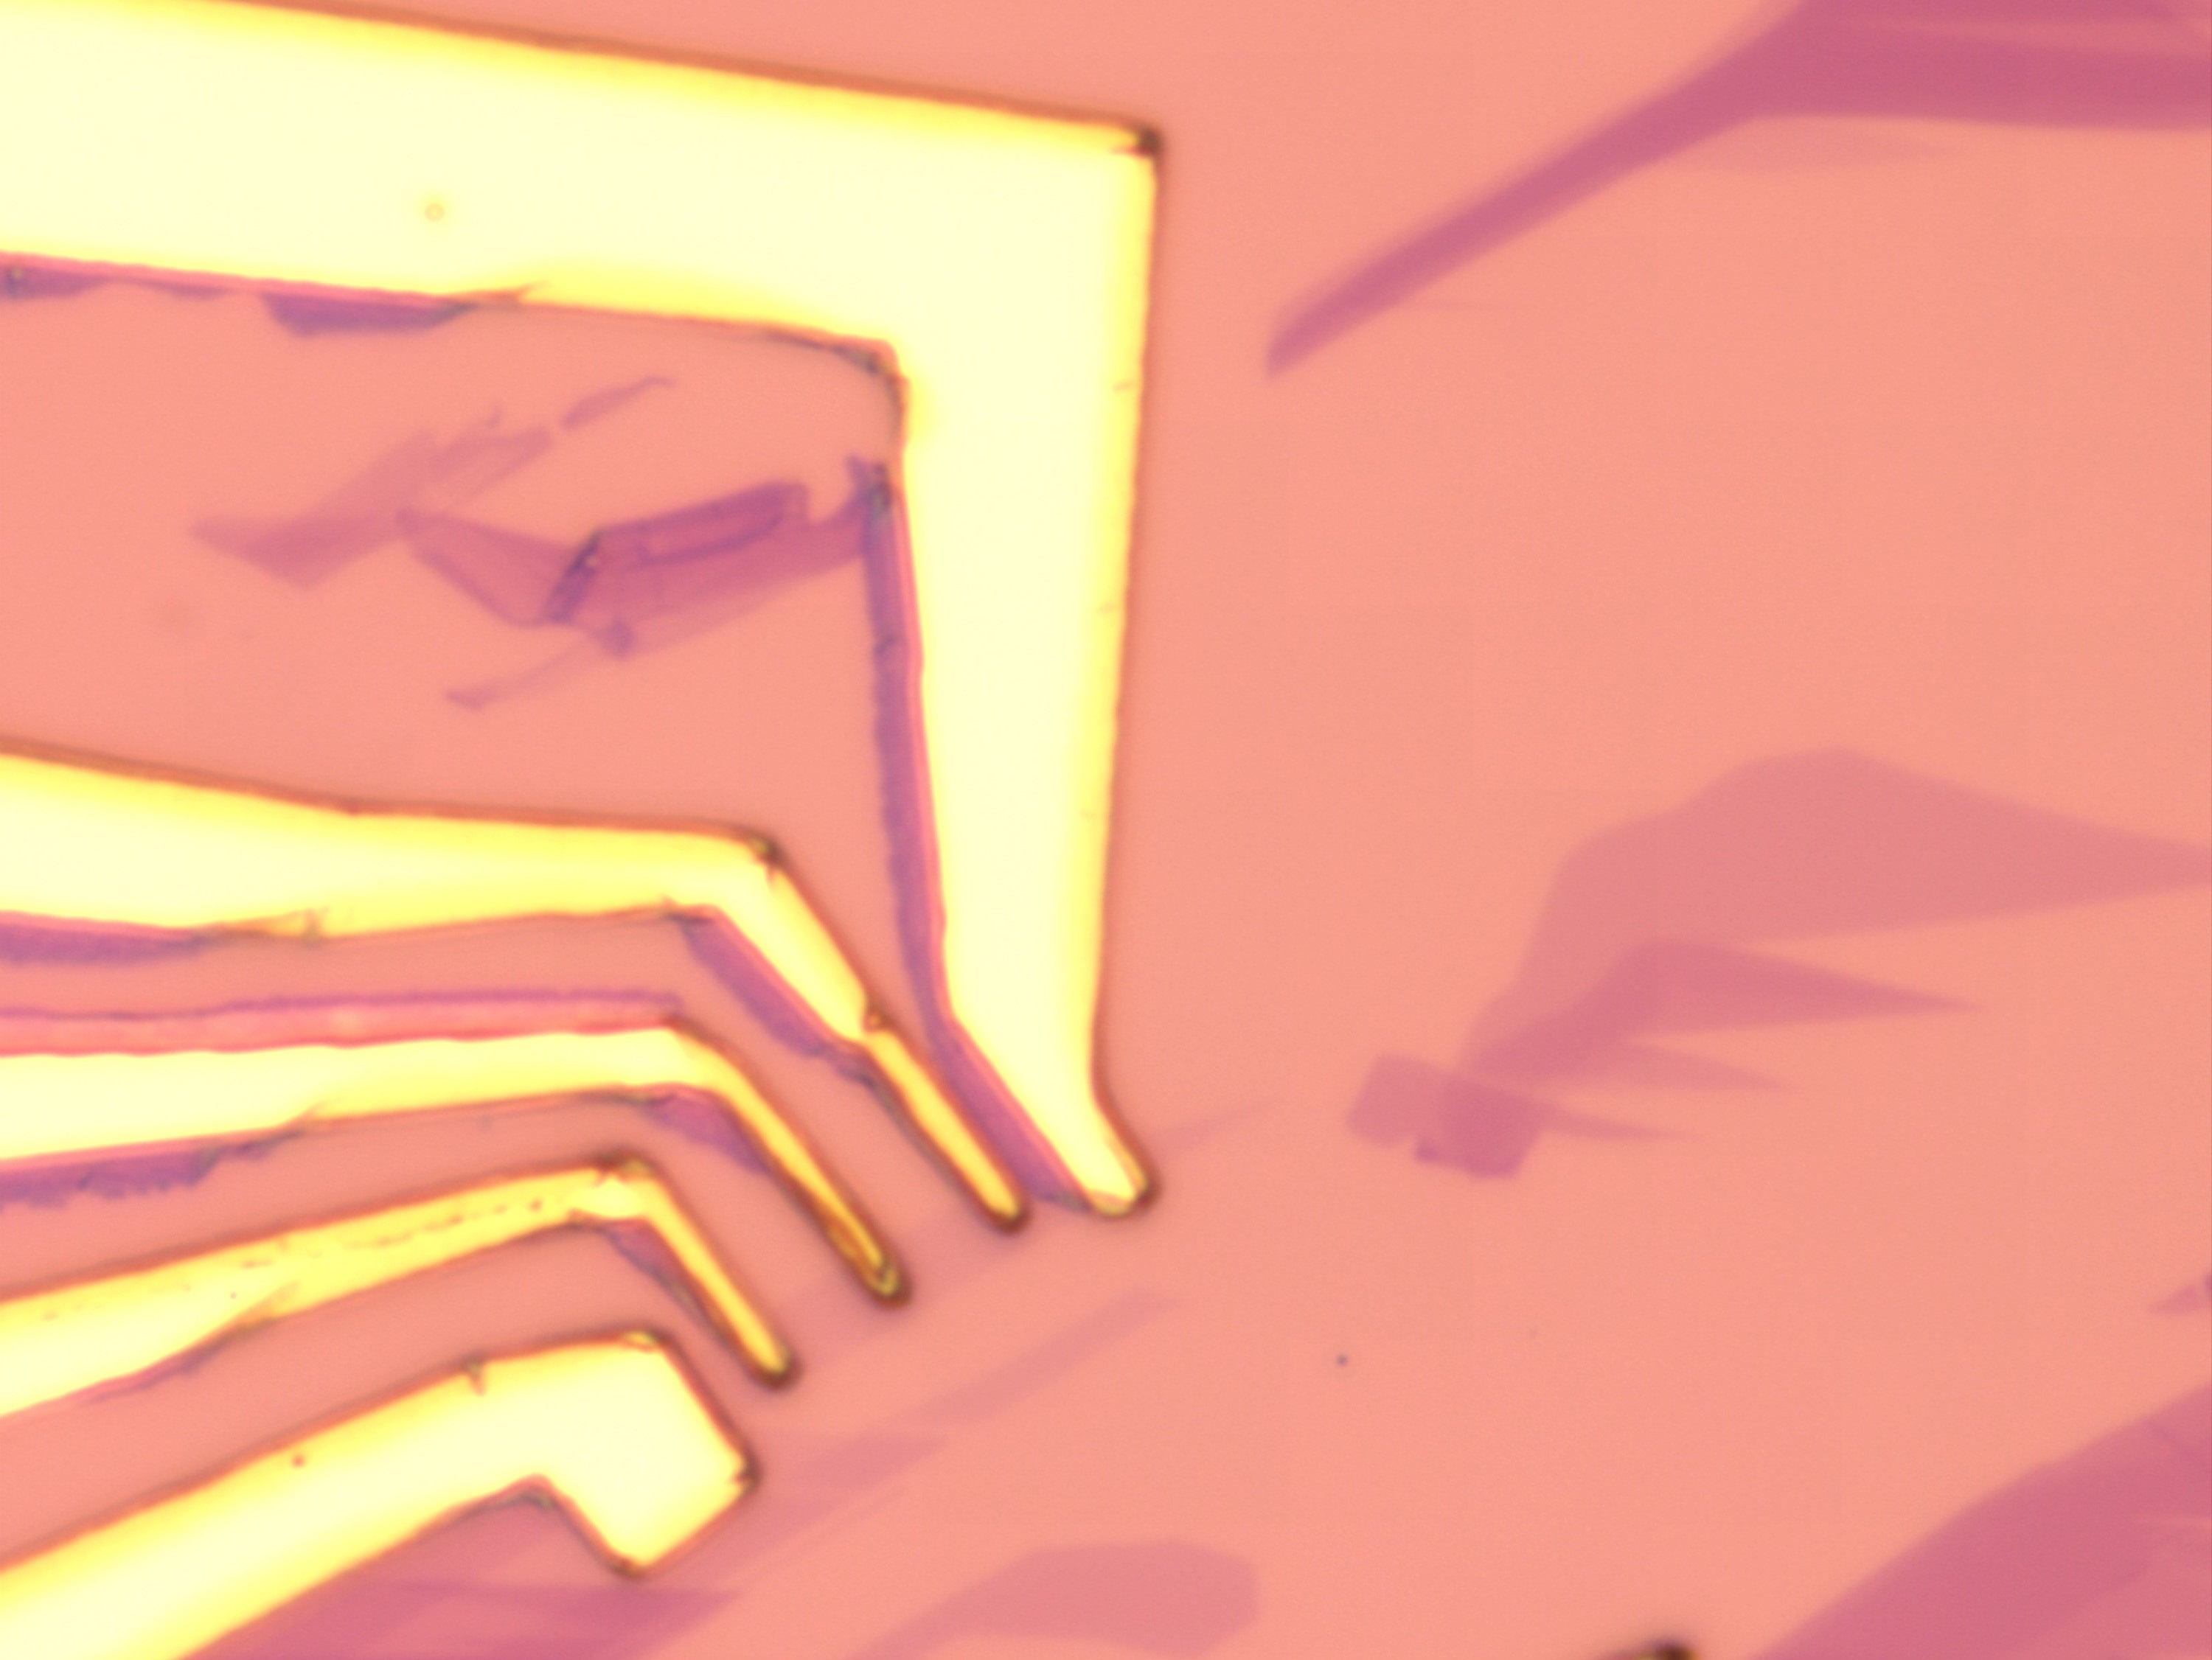
\includegraphics[width=\textwidth]{chap2/US/2_100x.jpg}
			\caption{After metal lift off}			
		\end{subfigure}
		\begin{subfigure}[b]{0.3\textwidth}
			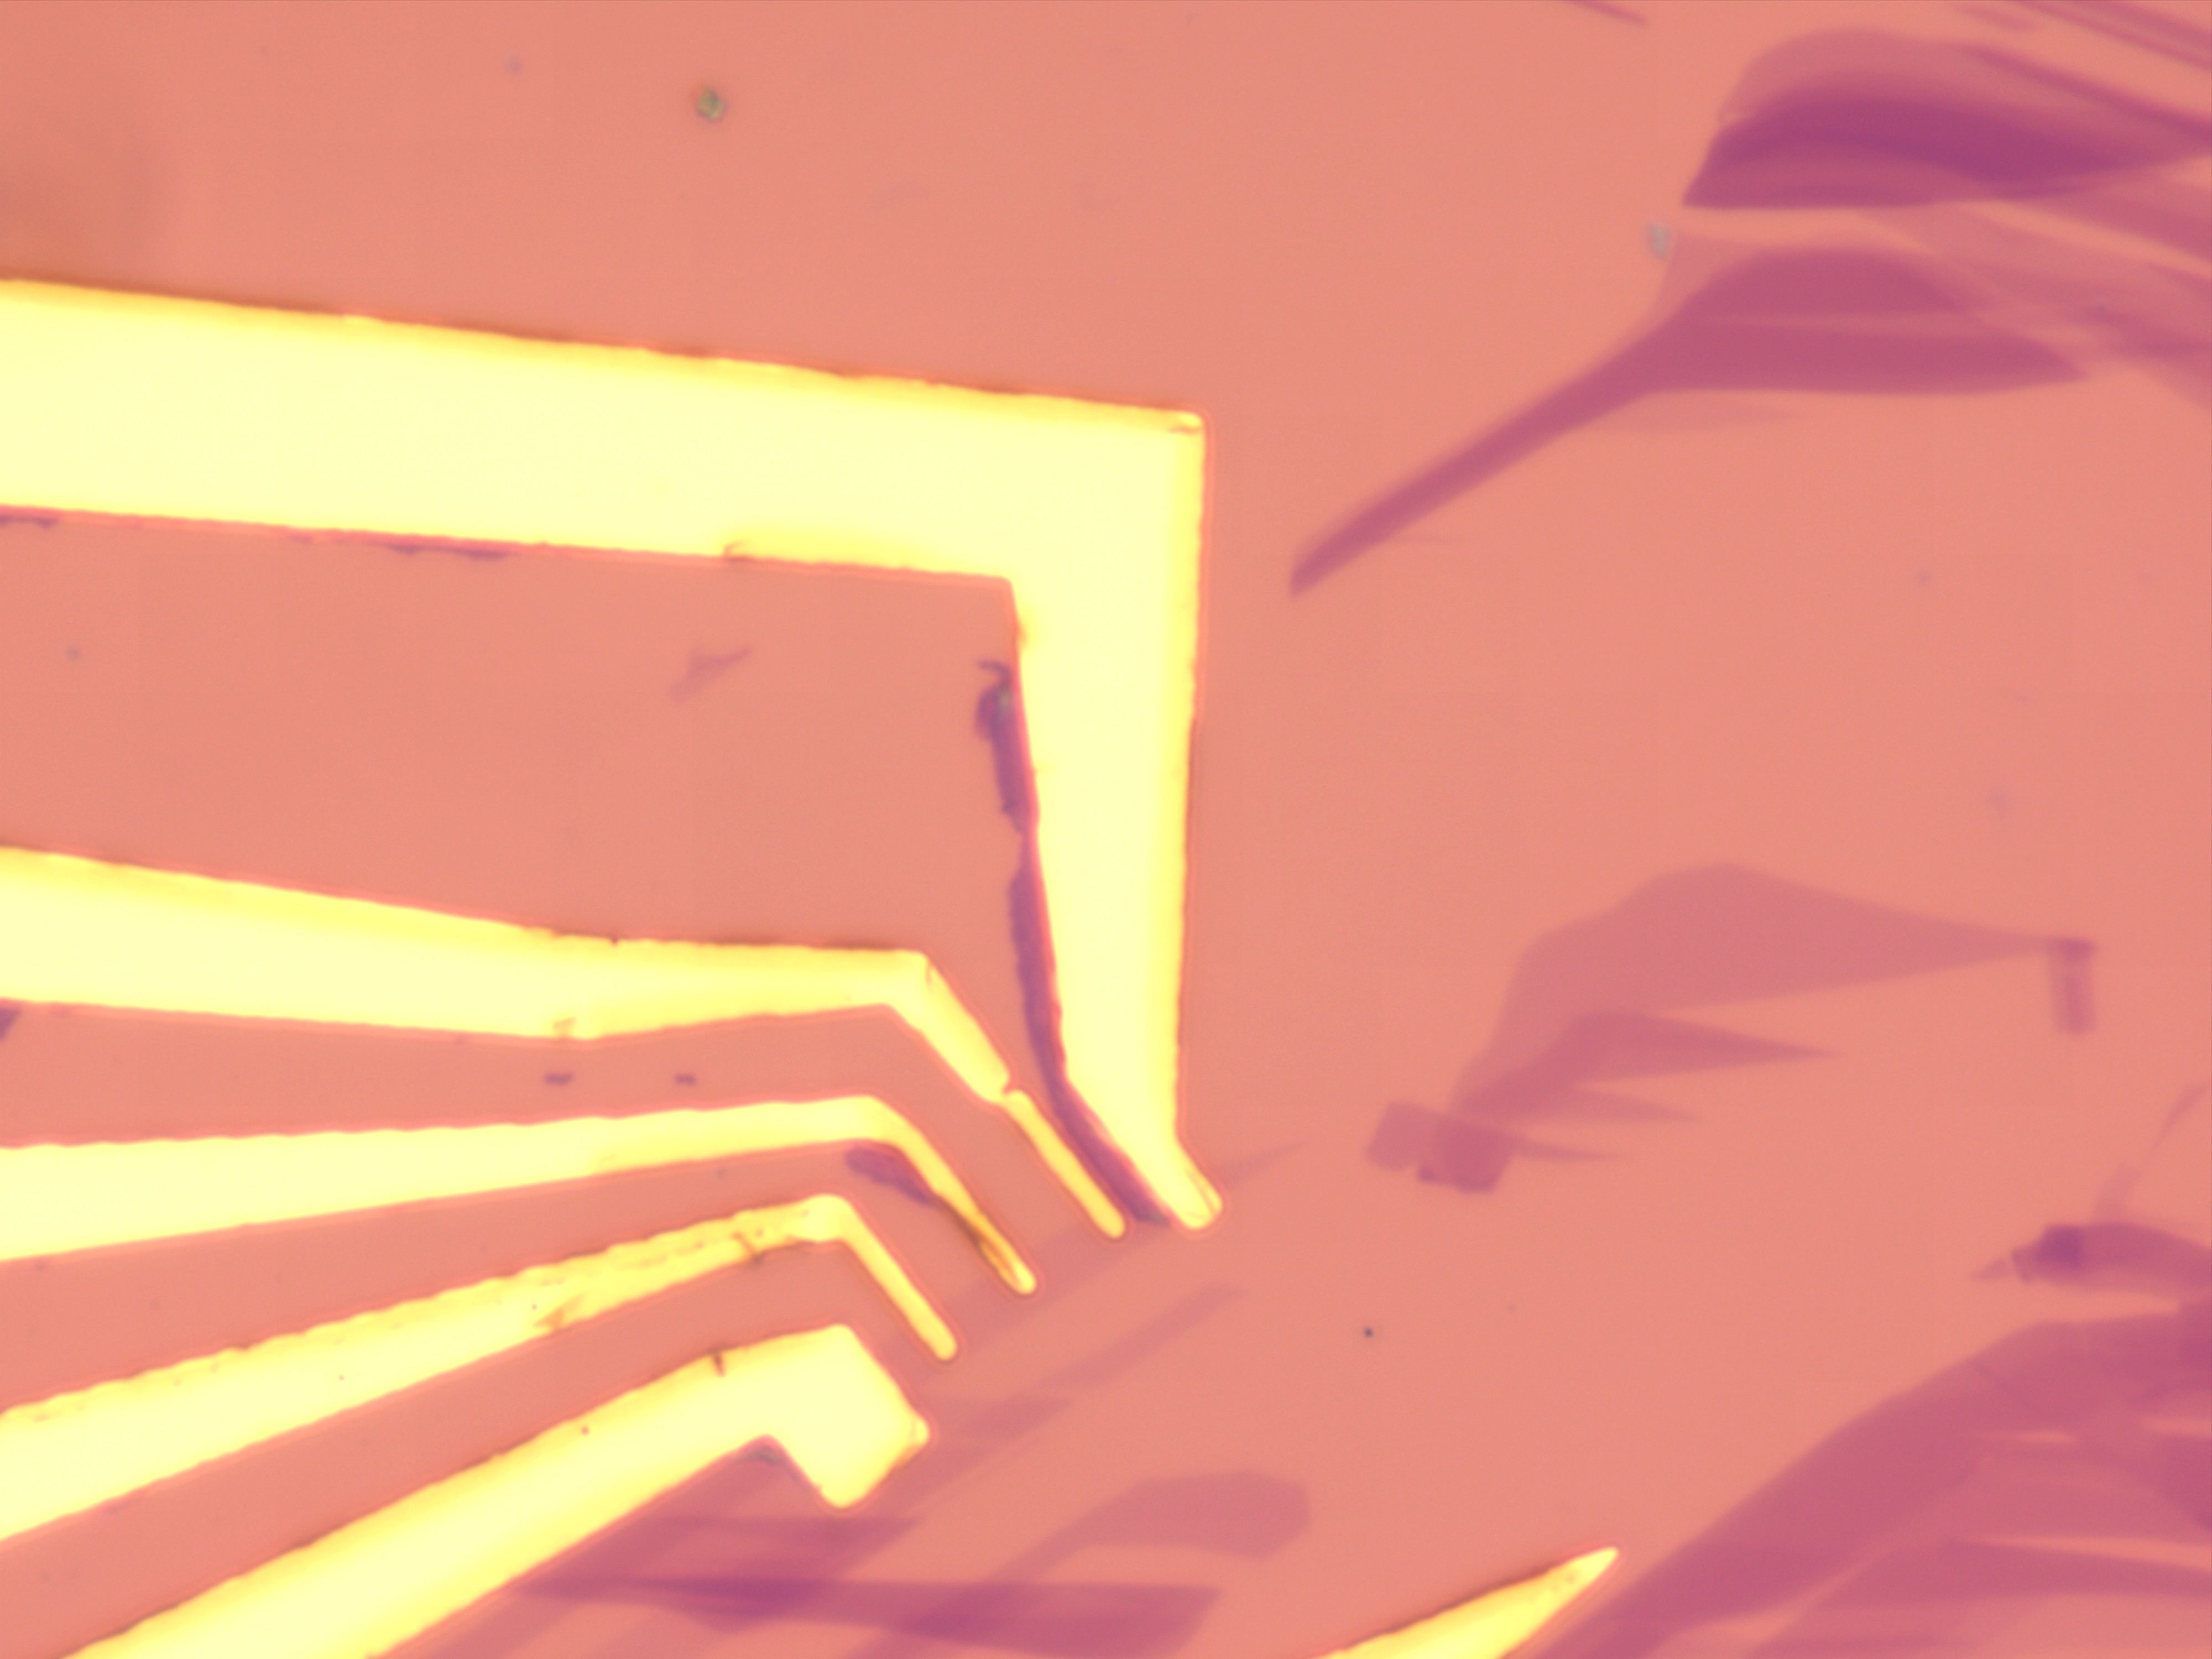
\includegraphics[width=\textwidth]{chap2/US/2_100x_after6sAcetoneUS.jpg}
			\subcaption{after 5s ultrasonication}
		\end{subfigure}
		\begin{subfigure}[b]{0.3\textwidth}
			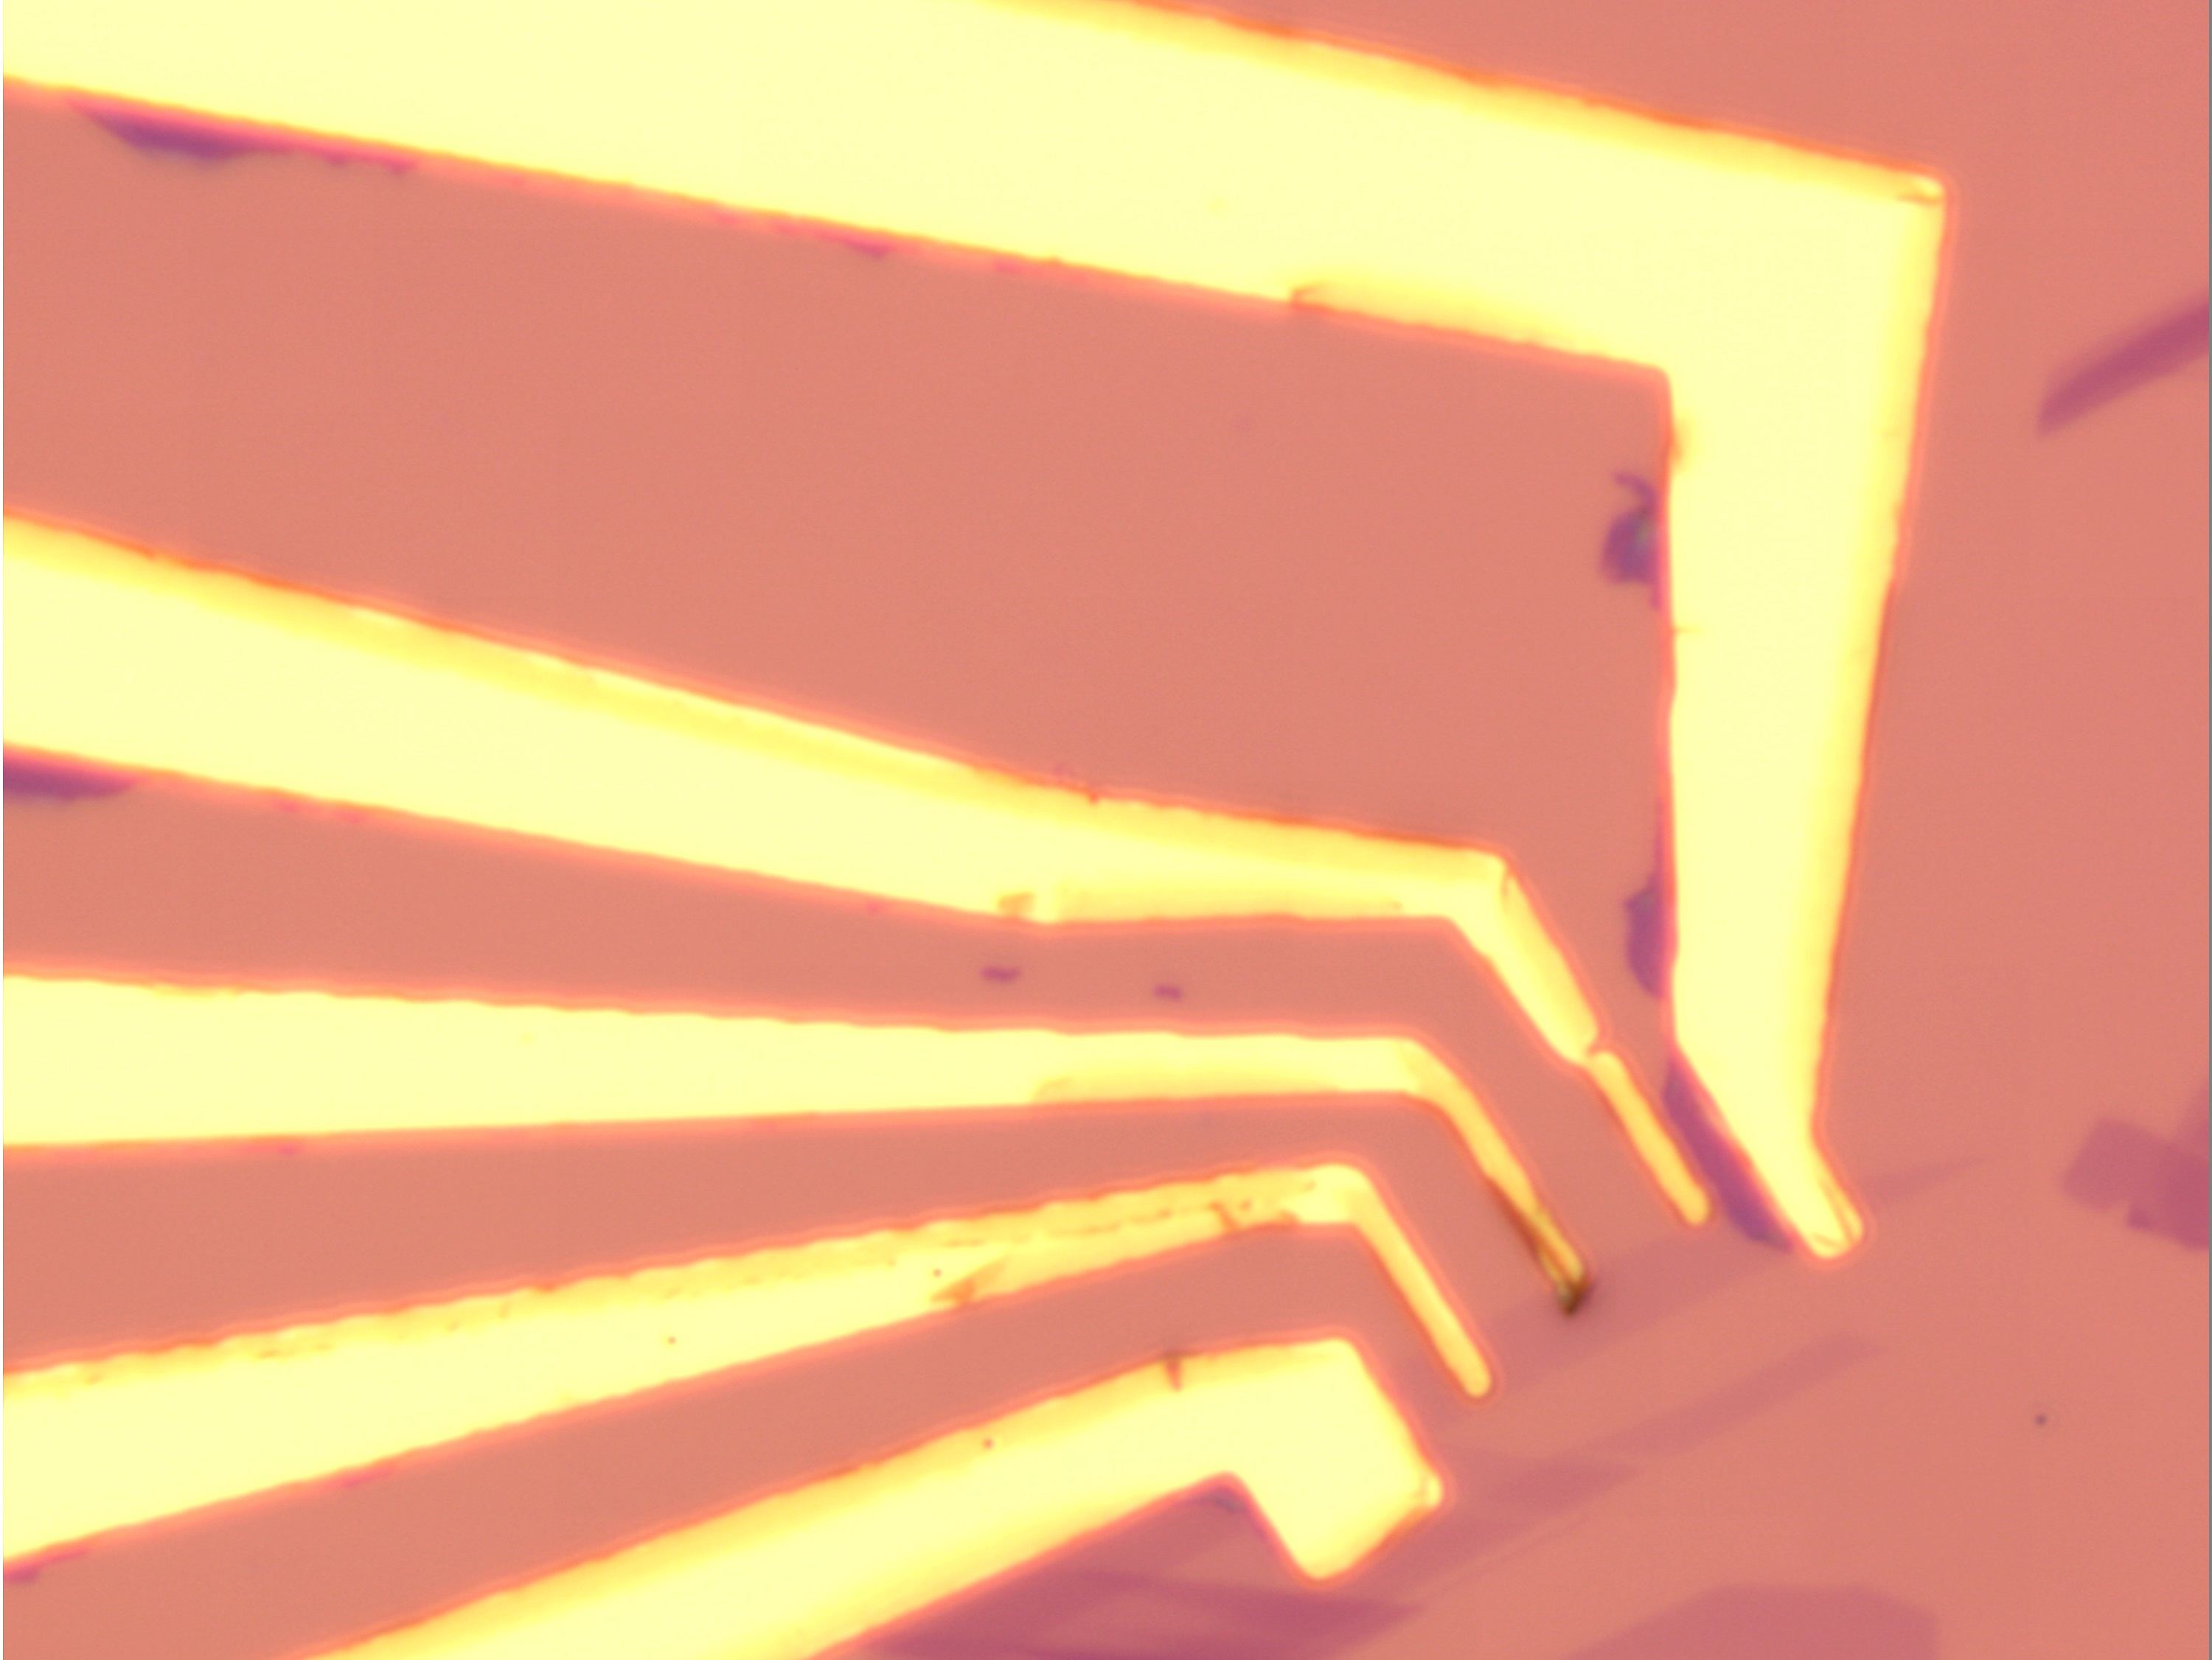
\includegraphics[width=\textwidth]{chap2/US/2_100x_after10sAcetoneUS.jpg}
			\subcaption{after 10s ultrasonication}		
		\end{subfigure}
		\caption{Ultrasonication used to remove material remanants from lithography.}\label{fig:lithography_skins_us}Note the movement or loss of gold material on the middle probes.
	\end{figure}
	
	\begin{figure}[H]
		\centering
		\begin{subfigure}[b]{0.3\textwidth}
			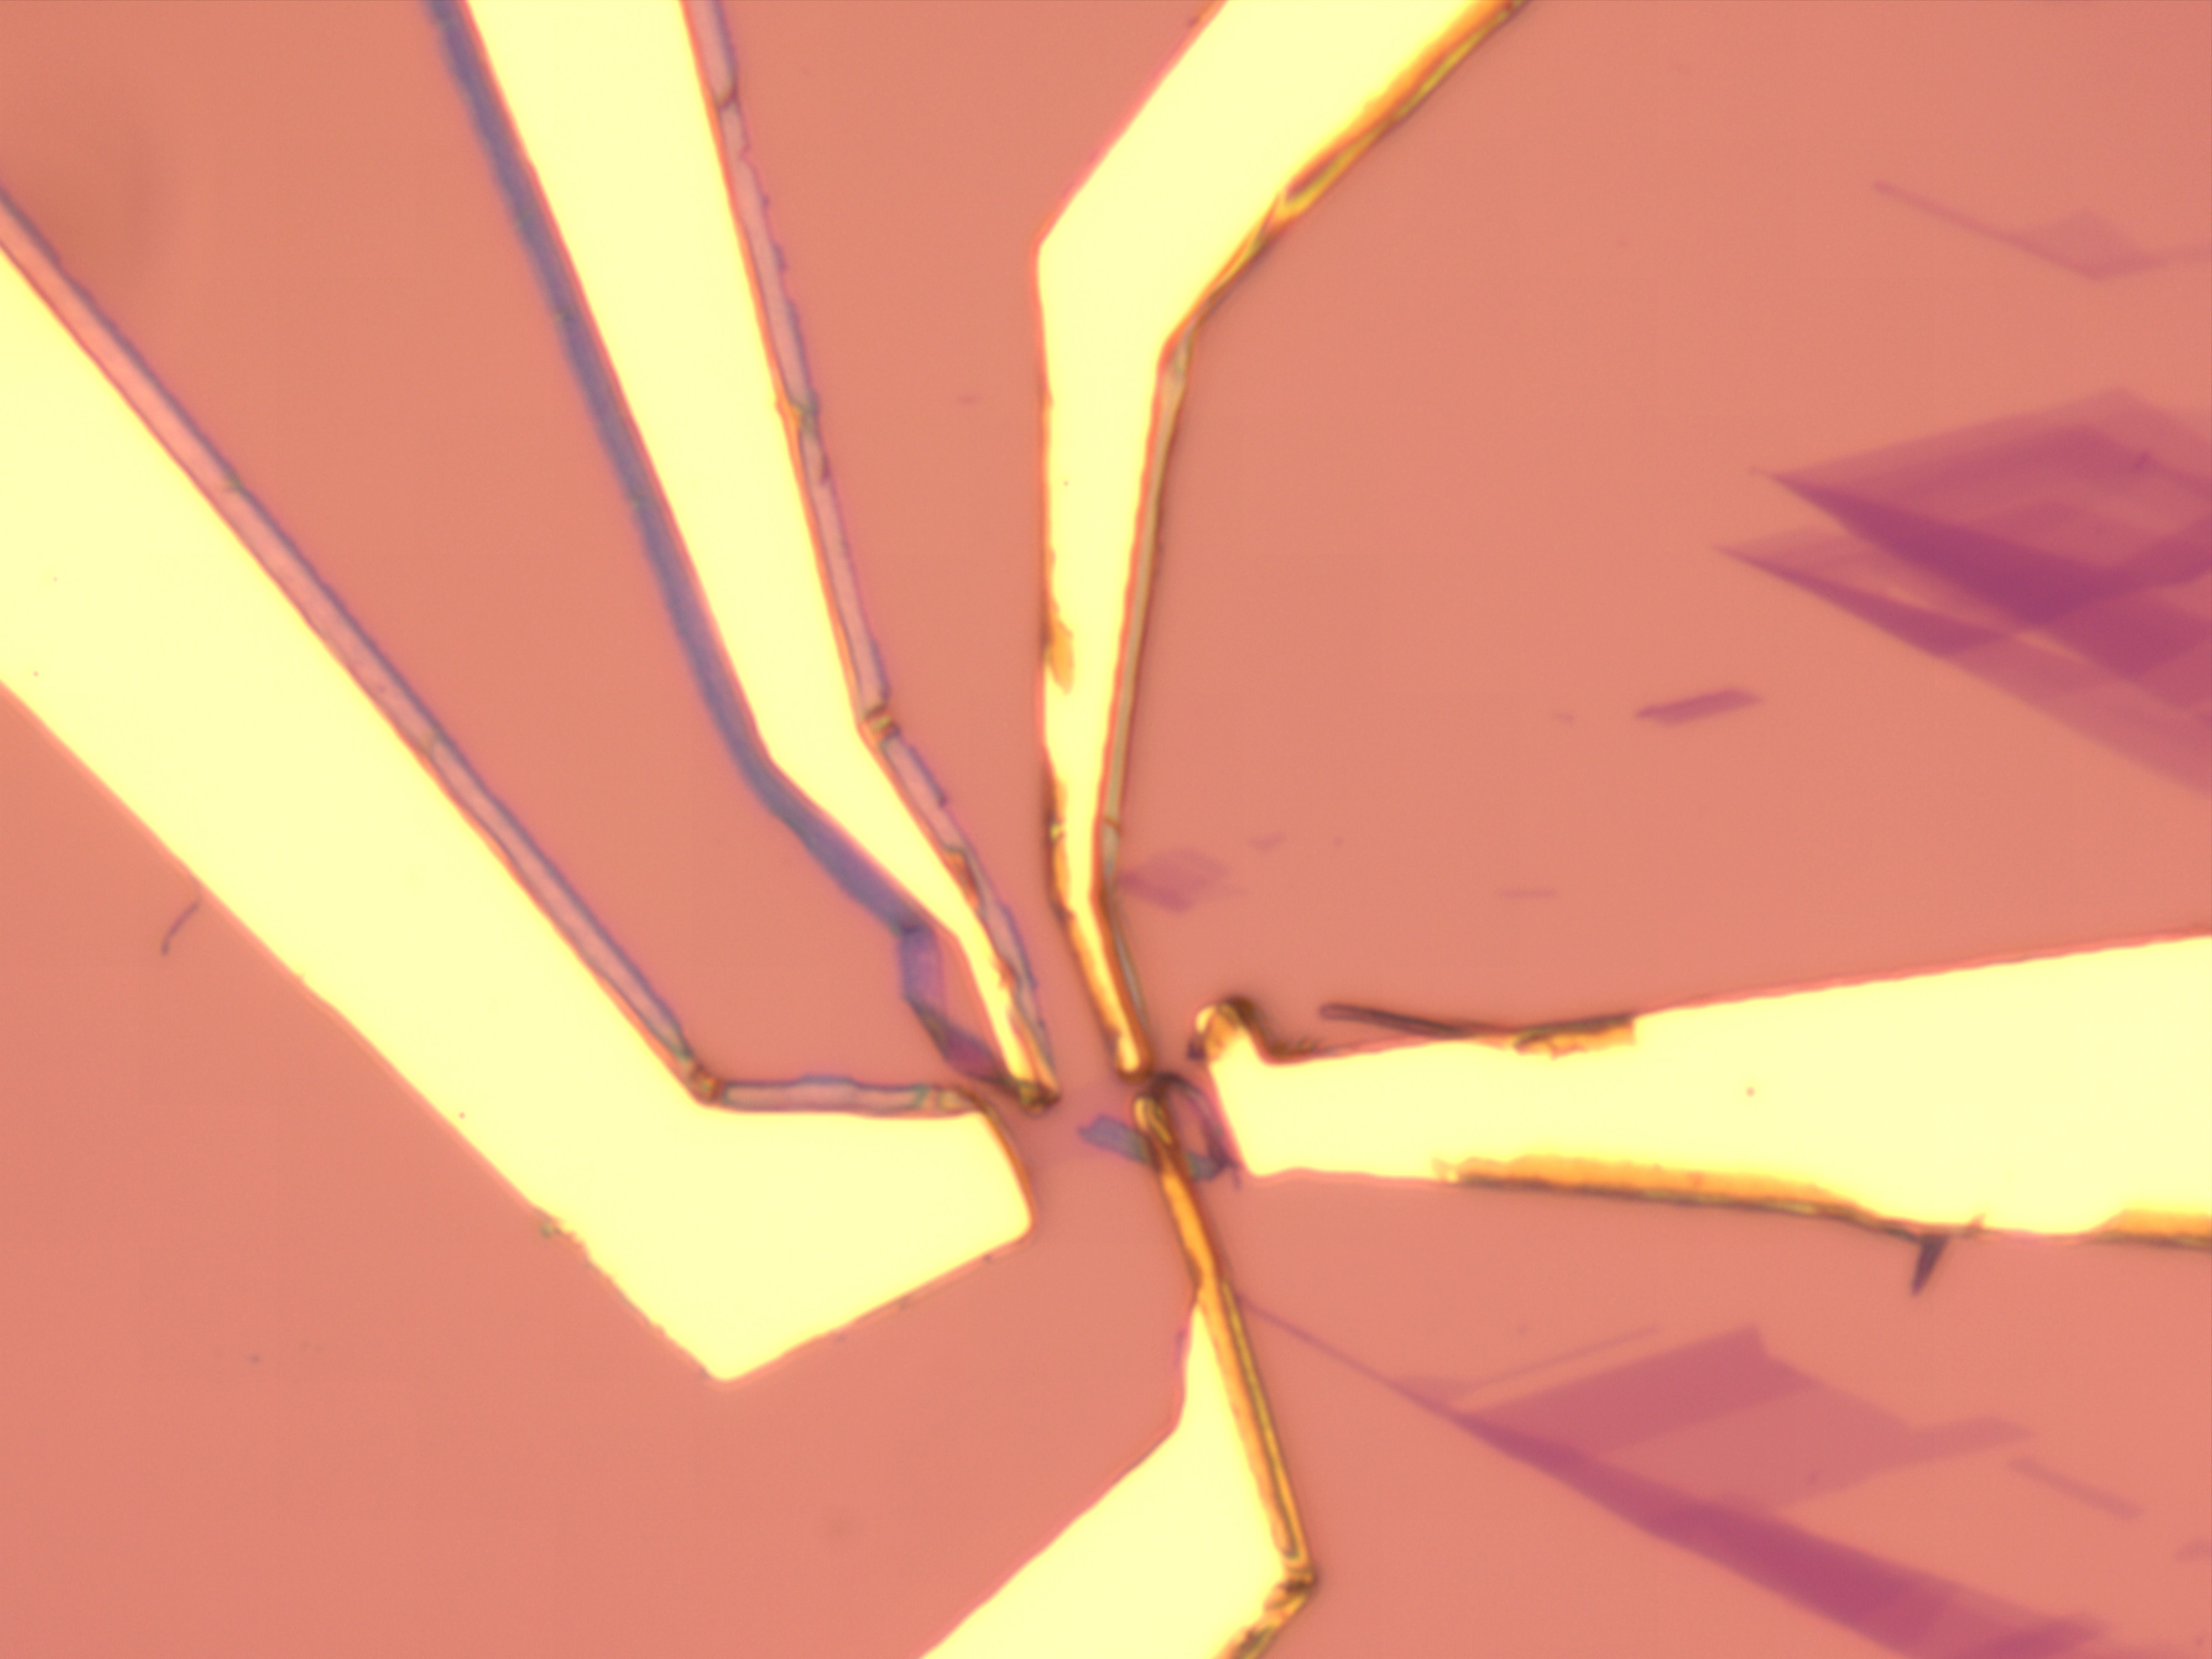
\includegraphics[width=\textwidth]{chap2/US/1_a}
			\caption{After metal lift off}
		\end{subfigure}
		\begin{subfigure}[b]{0.3\textwidth}
			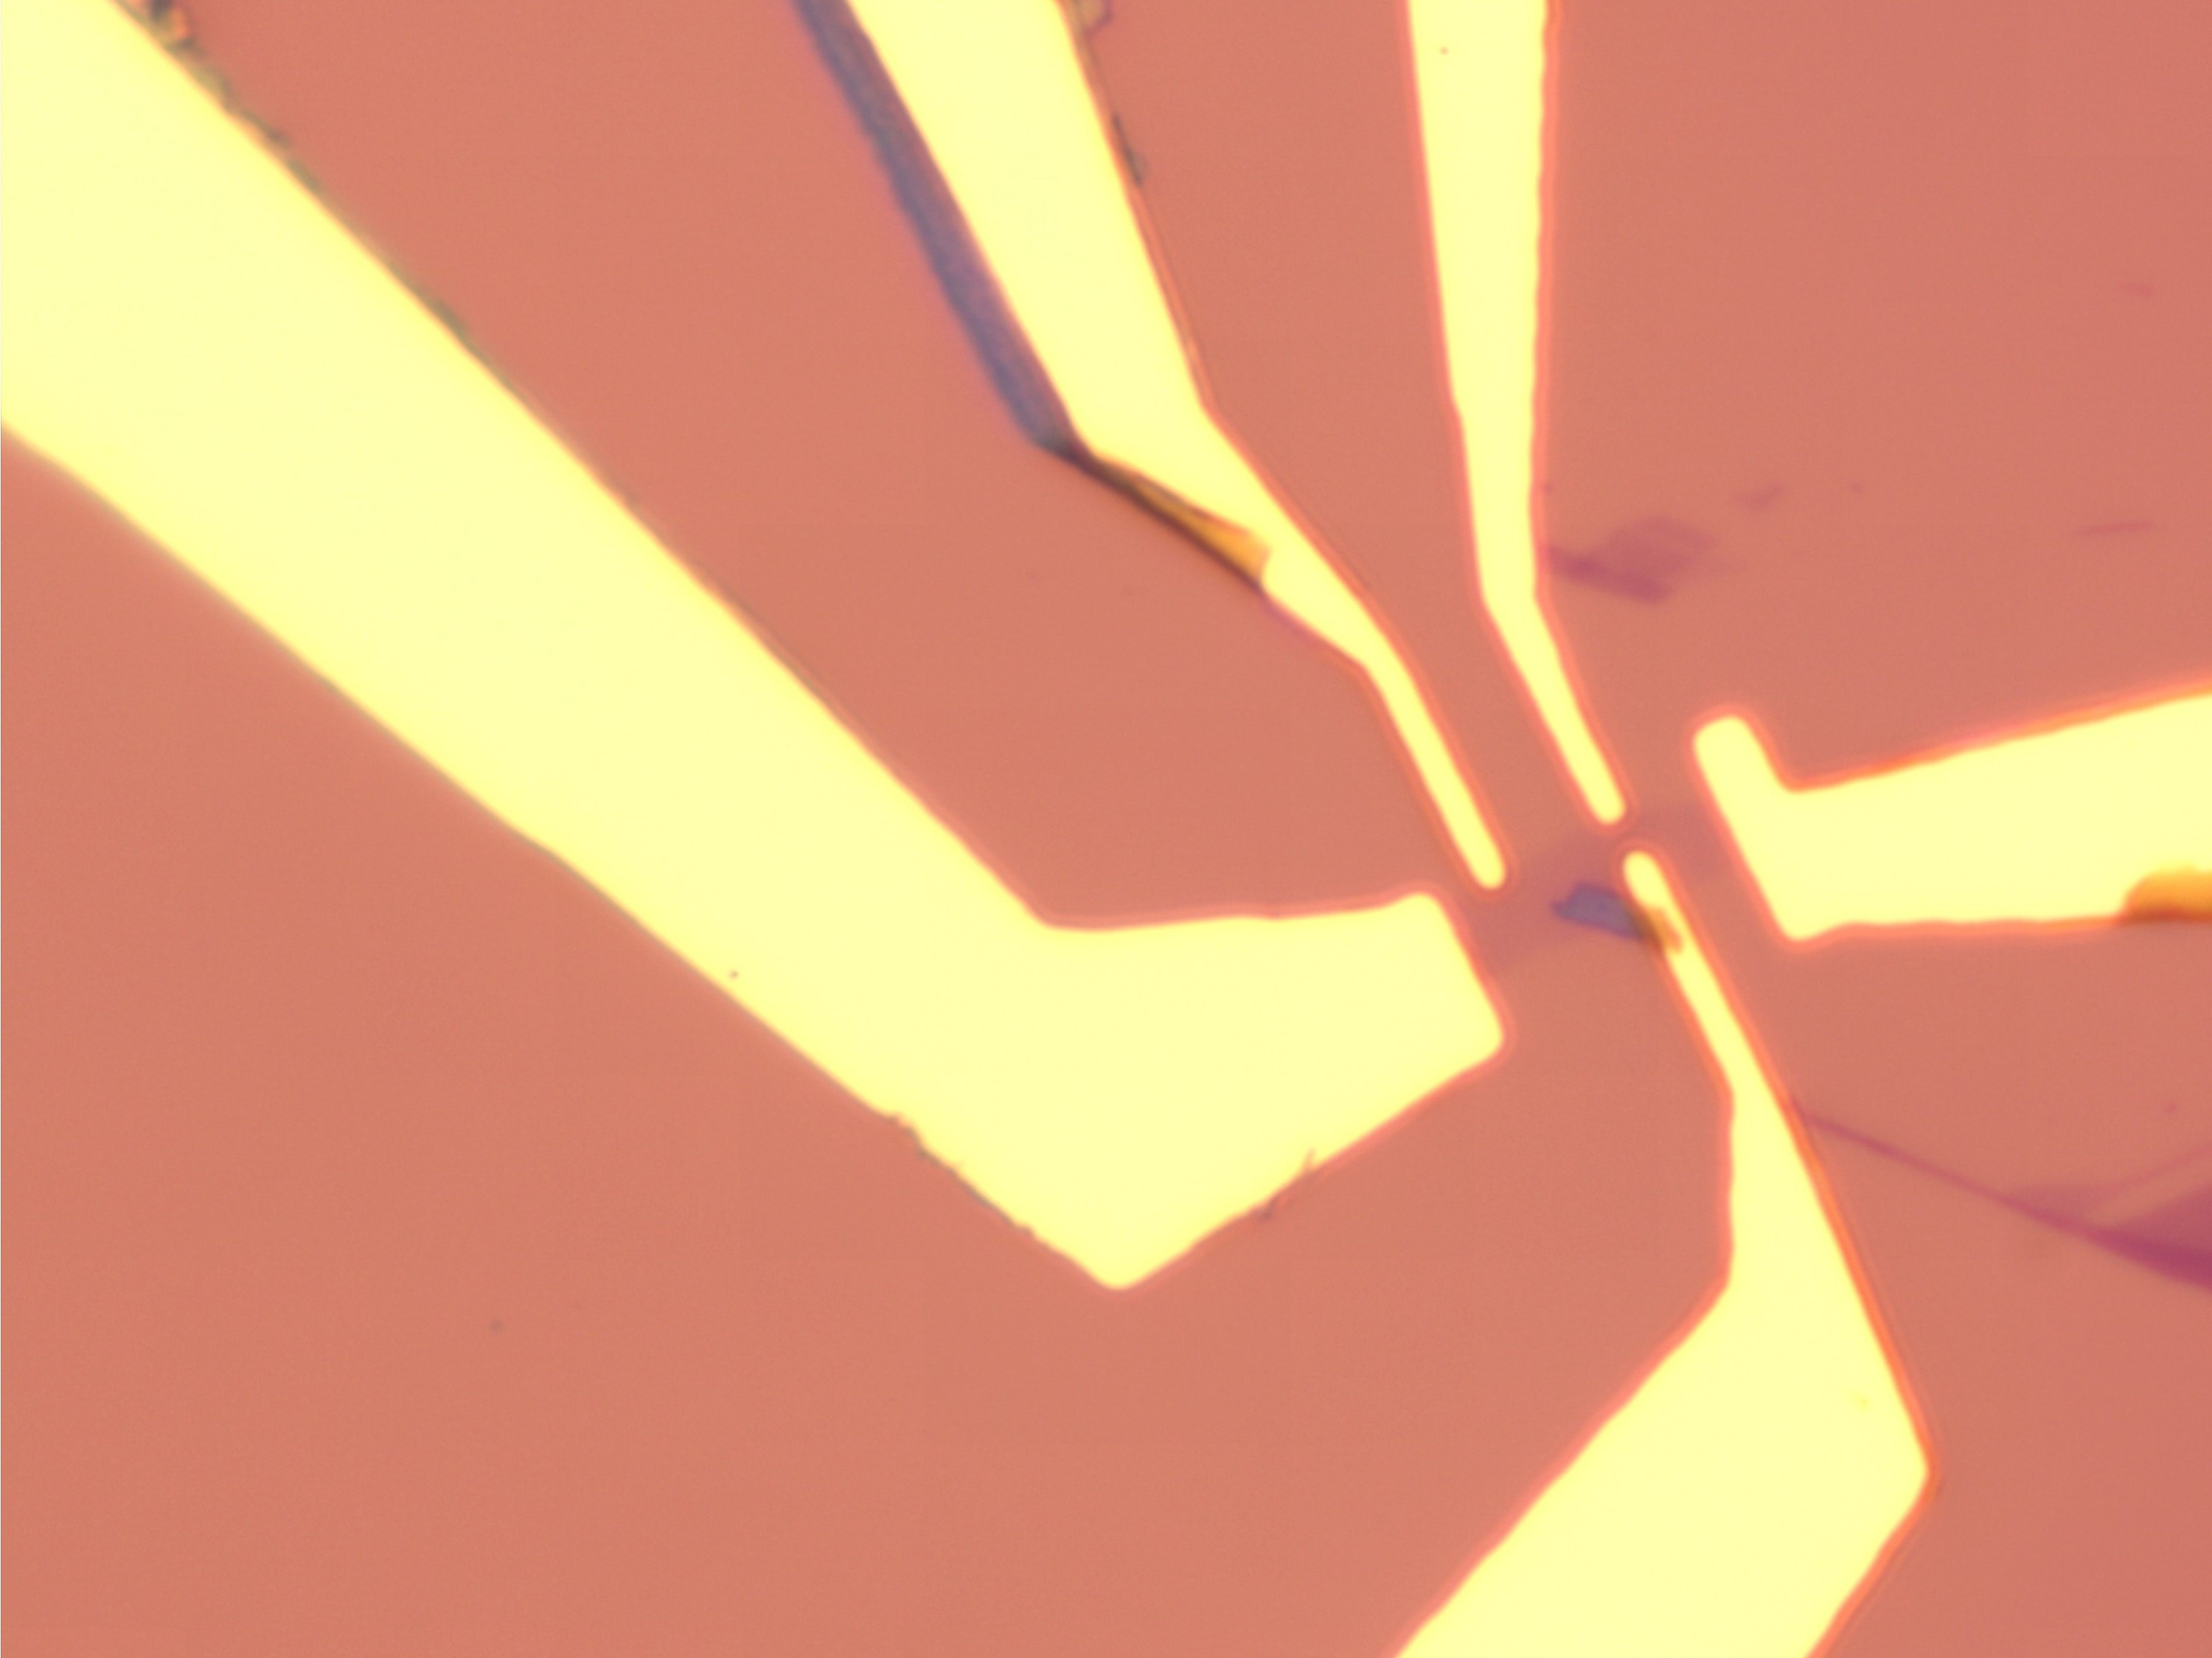
\includegraphics[width=\textwidth]{chap2/US/1_b}
			\caption{After 4s ultrasonication}
		\end{subfigure}
		\begin{subfigure}[b]{0.3\textwidth}
			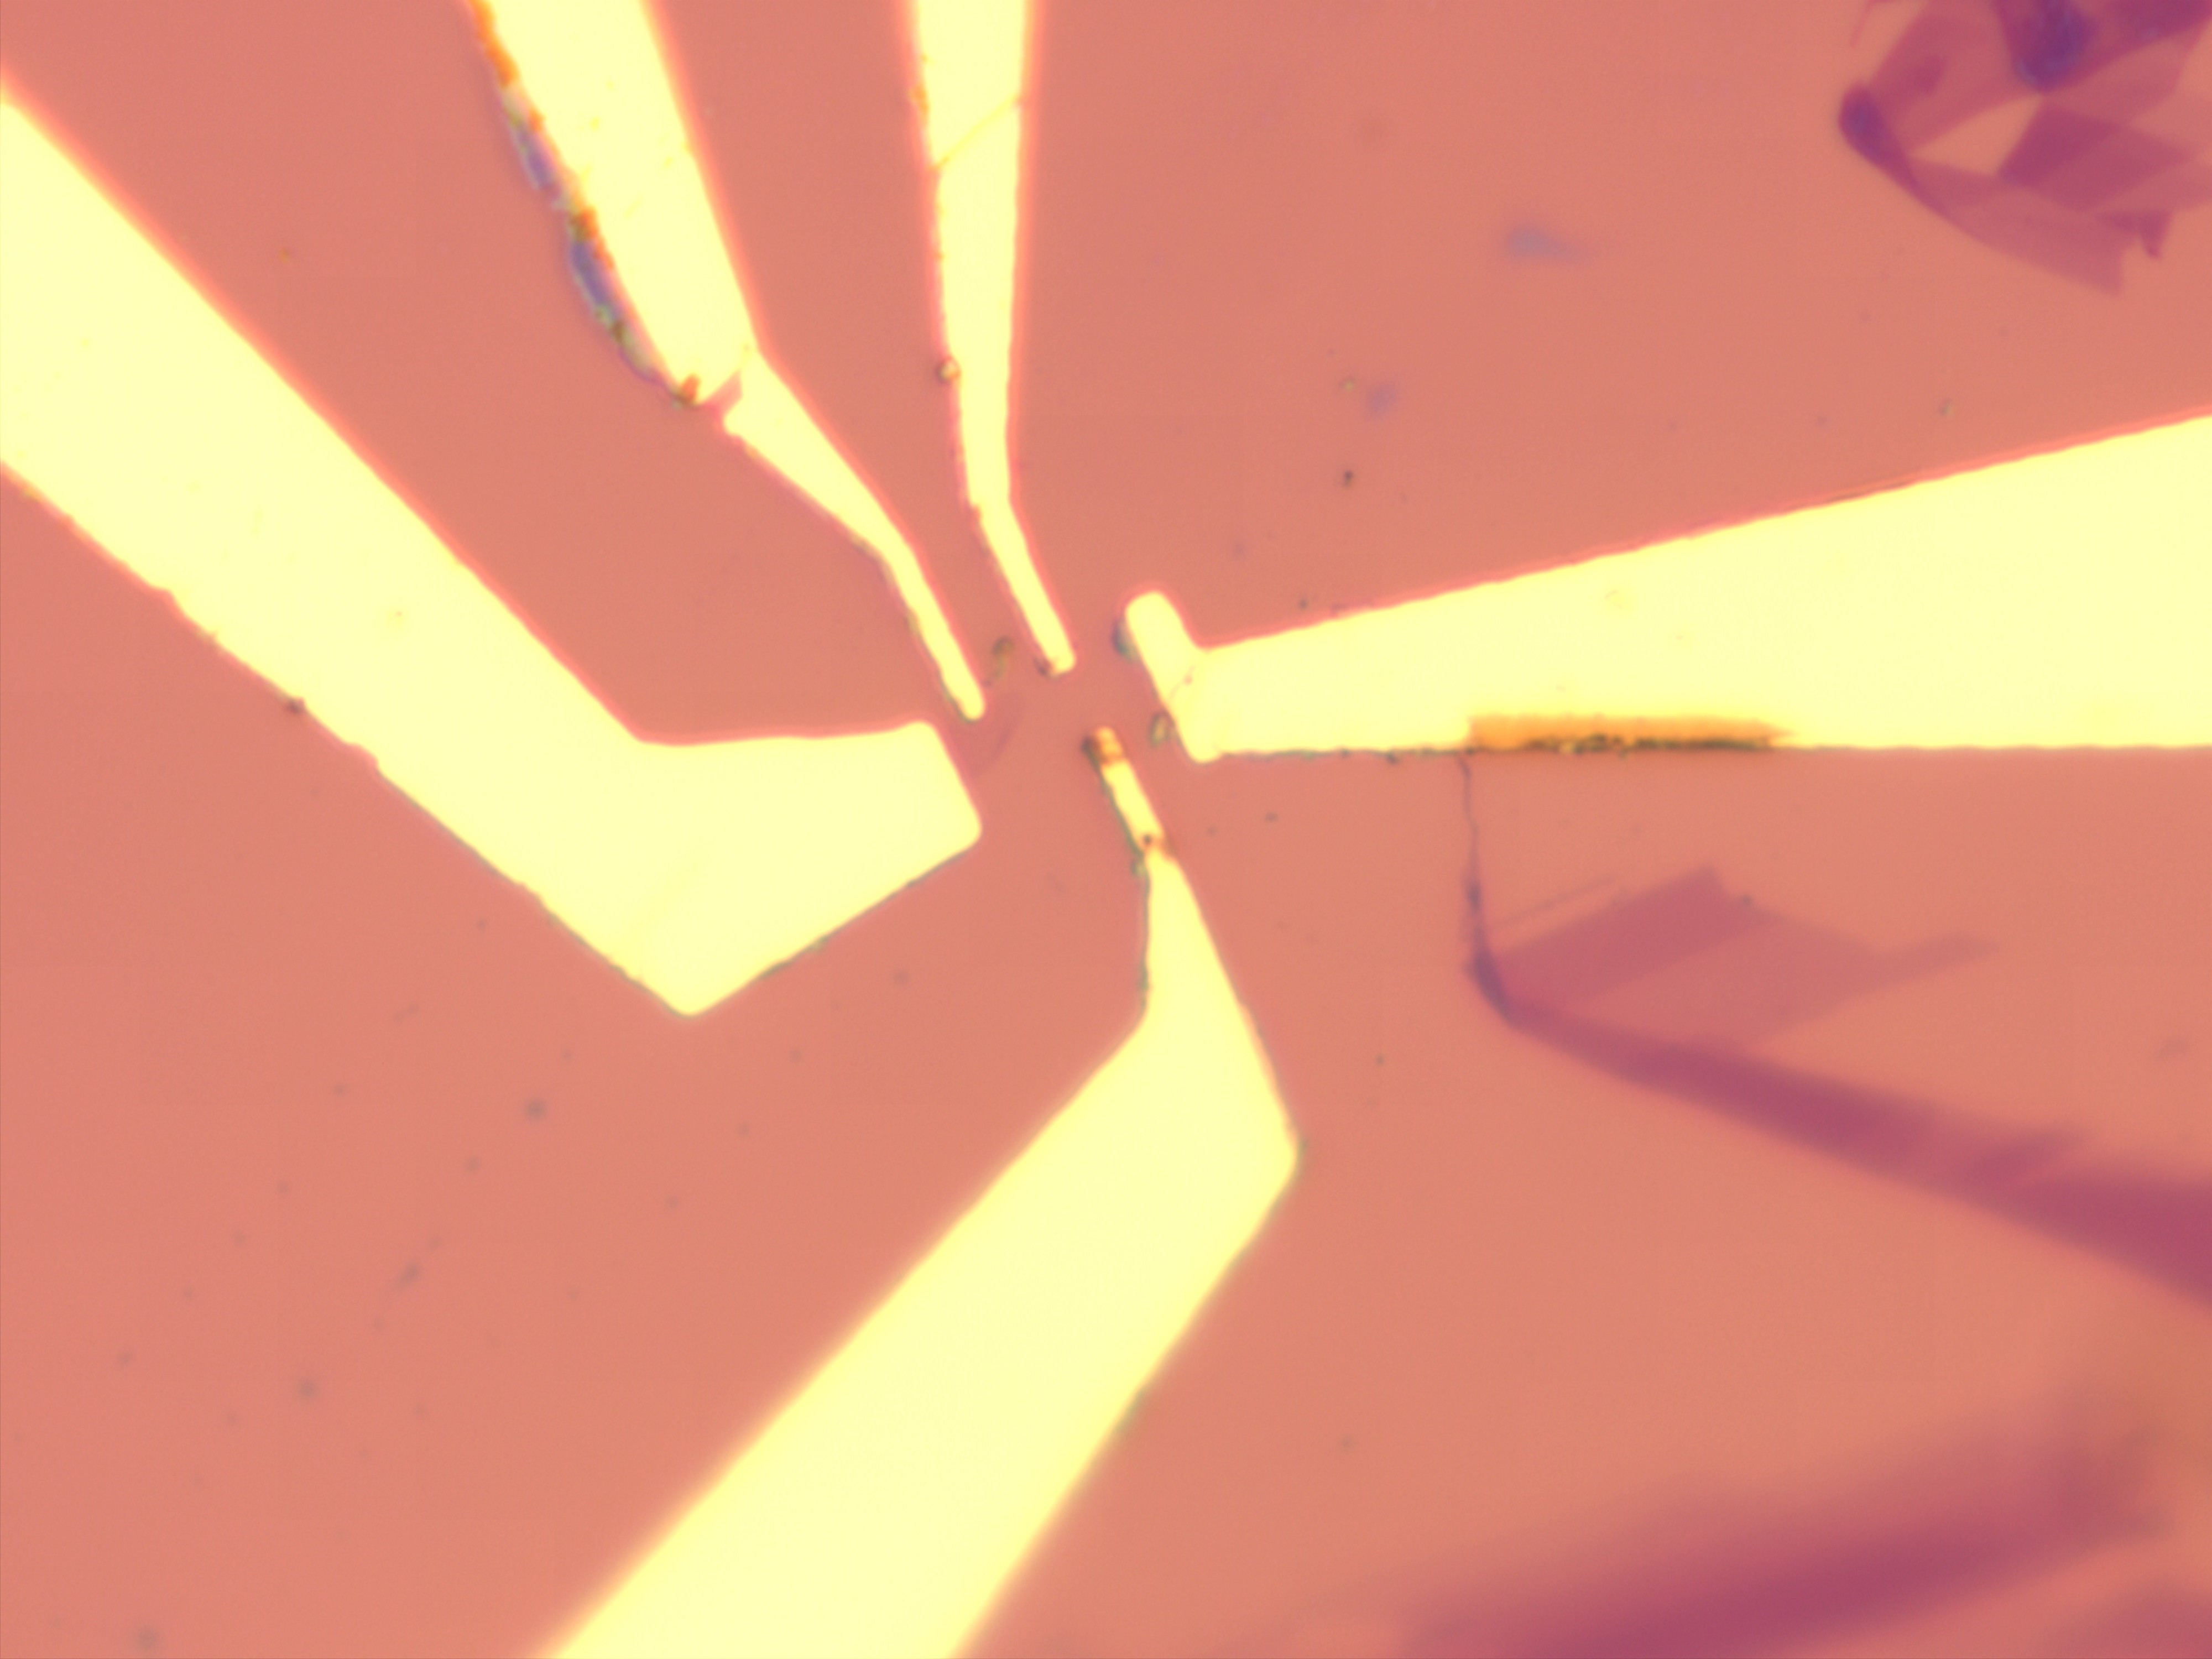
\includegraphics[width=\textwidth]{chap2/US/1_c}
			\caption{After 6s ultrasonication}
		\end{subfigure}
		\caption{Ultrasonication that has broken graphene sample.}\label{fig:lithography_skins_break}
	\end{figure}

	\subsection{Oxide stamping}
	% Introduction to metal stamping technique. Don't talk about optimisation here.
	Zavabeti \etals\cite{zavabeti_liquid_2017} work on thin oxides synthesised by liquid metal introduces two methods to create such oxides. The first involves the exfoliation of oxide layers from the surface of metal droplets, and the second involves the suspension of oxide layers in water, created by injecting gas through the metal liquid. This section will only describe the former in detail, which is used in this project. Refer to \cref{chap:thinoxides} for further optimisation and exploration of the liquid metal technique.
	
	\begin{figure}[H]
		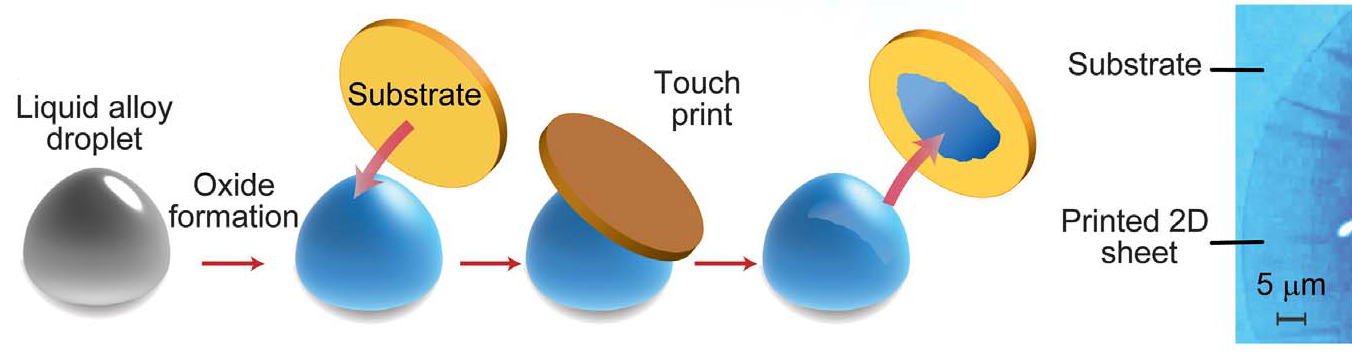
\includegraphics[width=\textwidth]{chap2/liq_metal_exfol}
		\caption{Process of liquid metal oxide exfoliation (source: Zavabeti \etal{}\cite{zavabeti_liquid_2017})}\label{fig:liq_metal_exfoliation}
	\end{figure}	
	
	A eutectic gallium melt is made by combining elements such as gallium, indium and tin. At room temperature these alloys are metallic liquids, and form atomically thin oxides on their surfaces. Because the formation of oxides change the Gibbs free energy of the system, those that provide the greatest reduction dominate the surface\cite{zavabeti_liquid_2017}. After the melt is formed and exposed to oxygen for some time, the oxide is isolated by a van der Waals exfoliation technique, touching the liquid metal droplet to the solid substrate, as seen in \cref{fig:liq_metal_exfoliation}.
	
	For the primary example of creating \aluminimumoxide, aluminium pieces are cleaned using a tissue, before being cut up into a few mm long segments. After heating a gallium based melt into a liquid inside a glovebox with roughly 0.2-0.3\% oxygen, the gallium and aluminium are ground together using a mortar and pestle. 
	
\end{document}